%%%%%%%%%%%%%%%%%%%%%%%%%%%%%%%%%%%%%%%%%%%%%%%%%%%%%%%%%%%%%%%%%%%%%%
% Universidade Federal de Santa Catarina
% Biblioteca Universitária
%
% (c)2010 Roberto Simoni (roberto.emc@gmail.com)
%         Carlos R Rocha (cticarlo@gmail.com)
%%%%%%%%%%%%%%%%%%%%%%%%%%%%%%%%%%%%%%%%%%%%%%%%%%%%%%%%%%%%%%%%%%%%%%%
%\PassOptionsToPackage{abnt-etal-cite=1, abnt-etal-list=0}{abntcite}
\documentclass{ufscThesis}

%%%%%%%%%%%%%%%%%%%%%%%%%%%%%%%%%%%%%%%%%%%%%%%%%%%%%%%%%%%%%%%%%%%%%%%
% Pacotes usados especificamente para este documento
% Definidos pelo criador do documento
%%%%%%%%%%%%%%%%%%%%%%%%%%%%%%%%%%%%%%%%%%%%%%%%%%%%%%%%%%%%%%%%%%%%%%%
\usepackage{booktabs}
\usepackage{multirow}
\usepackage{graphicx}
\usepackage[ruled]{algorithm2e}
\usepackage[table,xcdraw]{xcolor}
\usepackage{lipsum}
\usepackage{amsmath}
\usepackage{amsfonts}
\usepackage{url}
\usepackage{rotating}
\usepackage{float}
\usepackage{pdfpages}
%%%%%%%%%%%%%%%%%%%%%%%%%%%%%%%%%%%%%%%%%%%%%%%%%%%%%%%%%%%%%%%%%%%%%%%
% Pacotes usados especificamente para este documento
% Definidos pelo AUTOR
%%%%%%%%%%%%%%%%%%%%%%%%%%%%%%%%%%%%%%%%%%%%%%%%%%%%%%%%%%%%%%%%%%%%%%%
\usepackage[printonlyused, withpage]{acronym}
\usepackage{subfigure}

%%%%%%%%%%%%%%%%%%%%%%%%%%%%%%%%%%%%%%%%%%%%%%%%%%%%%%%%%%%%%%%%%%%%%%%
% Comandos usados especificamente para este documento
% Definidos pelo AUTOR
%%%%%%%%%%%%%%%%%%%%%%%%%%%%%%%%%%%%%%%%%%%%%%%%%%%%%%%%%%%%%%%%%%%%%%%
\newcommand\todo[1]{\textcolor{red}{TODO: #1}}

%%%%%%%%%%%%%%%%%%%%%%%%%%%%%%%%%%%%%%%%%%%%%%%%%%%%%%%%%%%%%%%%%%%%%%%

%\renewcommand{\theequation}{\arabic{equation}} %se desejar tirar o capitulo

%\usepackage[labelsep=period]{caption} % O separador de legenda é um .
\usepackage[labelsep=endash]{caption} % O separador de legenda é um -

%%%%%%%%%%%%%%%%%%%%%%%%%%%%%%%%%%%%%%%%%%%%%%%%%%%%%%%%%%%%%%%%%%%%%%%
% Identificadores do trabalho
% Usados para preencher os elementos pré-textuais
%%%%%%%%%%%%%%%%%%%%%%%%%%%%%%%%%%%%%%%%%%%%%%%%%%%%%%%%%%%%%%%%%%%%%%%
\titulo{Avaliação do impacto da organização dos dados em Physical Design}
%\subtitulo{Estilo \LaTeX~ padrăo}                % Subtitulo do trabalho (opcional)
\autor{Tiago Augusto Fontana}                     % Nome do autor
\data{}{Novembro}{2017}                           % Data da publicaçăo do trabalho

\orientador{Prof.\ Dr.\ José\ Luís\ Almada\ Güntzel} % Nome do orientador e (opcional) seu título
%\coorientador{Prof. Dr. Beltrano}                % Nome do coorientador e seu título (opcional)
%\coordenador{Prof. Chefe, Dr. Eng.}              % Nome do coordenador do curso e (opcional) seu título

\departamento{Programa de Pós-Graduação em Ciência da Computação}
\curso{Programa de Pós-Graduação em Ciência da Computação}

\documento[a]{Dissertação}
\grau{Mestre em Ciência da Computação}


%%% Sobre a Banca
\numerodemembrosnabanca{3} % Isso decide se haverá uma folha adicional
\orientadornabanca{sim} % Se faz parte da banca definir como sim
%\coorientadornabanca{sim} % Se faz parte da banca definir como sim
\bancaMembroA{Dr.\ José\ Luis\ Almada\ Güntzel} %Nome do presidente da banca
\bancaMembroB{Dr.\ }      % Nome do membro da Banca
\bancaMembroC{Dr.\ }       % Nome do membro da Banca
% \bancaMembroD{Dr.\ }     % Nome do membro da Banca
%\bancaMembroE{Prof. quinto membro}       % Nome do membro da Banca
%\bancaMembroF{Prof. sexto membro}        % Nome do membro da Banca
%\bancaMembroG{Prof. sétimo membro}       % Nome do membro da Banca

\dedicatoria{A quem o trabalho é dedicado, se é que o é (opcional)}

\agradecimento{Agradeço ao meu orientador José Luís Almada Güntzel, por todo o auxílio oferecido
na execução deste trabalho e na escrita deste texto. \\
Agradeço aos membros da banca, por cederem seu tempo para a avaliação deste trabalho. \\
% Agradeço aos meus colegas de trabalho Vinicius dos Santos Livramento e Chrystian de Sousa Guth,
% pela ajuda durante a realização deste trabalho. \\
% Agradeço à minha namorada Taciane Martimiano, por me acompanhar nestes dois anos de mestrado. \\
% Por fim, agradeço à minha família Carlos Alberto Barbosa Netto, Loreni Oliveira Netto e Caio Oliveira Netto,
% por todo apoio e dedicação oferecidos até hoje, pois sem eles, nada disso seria possível.
}

\epigrafe{Um bonito pensamento ou citaçăo, se for o caso}{autor do pensamento}

\textoResumo{ }

\palavrasChave{ }

\textAbstract{ }

\keywords{ }

%%%%%%%%%%%%%%%%%%%%%%%%%%%%%%%%%%%%%%%%%%%%%%%%%%%%%%%%%%%%%%%%%%%%%%%
% Início do documento
%%%%%%%%%%%%%%%%%%%%%%%%%%%%%%%%%%%%%%%%%%%%%%%%%%%%%%%%%%%%%%%%%%%%%%%
\begin{document}
%--------------------------------------------------------
% Elementos pré-textuais
\capa
%\folhaderosto[comficha] % Se nao quiser imprimir a ficha, é só năo usar o parâmetro
\folhaderosto% Se nao quiser imprimir a ficha, é só năo usar o parâmetro
% \includepdf[pages={1}]{capitulos/ficha_catalografica.pdf}
% \includepdf{capitulos/aprovacao.pdf}
%\paginadedicatoria
%\paginaagradecimento
%\paginaepigrafe
\paginaresumo
\paginaabstract
\listadefiguras
\listadetabelas
\begin{singlespacing}
\chapter * {Lista de Abreviaturas e Siglas}
\thispagestyle{empty}
\label{acro}
%\addcontentsline{toc}{chapter}{Lista de Acr�nimos}
%\begin{tabbing}

%\singlespace

\begin{acronym}
\setlength{\parskip}{0ex}
\setlength{\itemsep}{1ex}

%\begin{singlespace}

\renewcommand{\baselinestretch}{0.25}%
\large\normalsize%



% tiago
\acro{dme}[DME]{\textit{Deferred-Merge Embedding}}
\acro{ecl}[ECL]{Laboratório de ComputaçãSo Embarcada - \textit{Embedded Computing Lab}}
\acro{eda}[EDA]{Electronic Design Automation}
\acro{ics}[ICs]{Circuitos Integrados - \textit{Integrated Circuits}}
\acro{mmm}[MMM]{Método de Médias e Medianas - \textit{Method of Means and Medians}}
\acro{rgm}[RGM]{Adequação Geométrica Recursiva - \textit{Recursive Geometric Matching}}
\acro{vlsi}[VLSI]{\textit{Very-large-scale Integrated}}



% andre
\acro{3ccd}[3 CCD]{\textit{Three-CCD}}
\acro{a1csa}[A1CSA]{\textit{Add-One Carry-Select Adder}}
\acro{a1csah}[A1CSAH]{\textit{Hierarchical Add-One Carry-Select Adder}}
\acro{ads}[ADS]{\textit{Absolute Difference of Sums}}
\acro{anova}[ANOVA]{Análise de Variância - \textit{Analysis of Variance}}
\acro{aps}[APS]{\textit{Alternating pel-subsampling block matching algorithm}}
\acro{asic}[ASIC]{\textit{Application Specific Integrated Circuit}}
\acro{AVCHD}{\textit{Advanced Video Codec High Definition}}
\acro{b}[B]{Bipredito}
\acro{bdbr}[BDBR]{\textit{Bjontegaard Delta Bitrate}}
\acro{bdpsnr}[BDPSNR]{\textit{Bjontegaard Delta PSNR}}
\acro{bm}[BM]{\textit{Block Matching}}
\acro{ccd}[CCD]{Dispositivo de Carga-Acoplada - \textit{Charge-Coupled Device}}
\acro{cla}[CLA]{\textit{Carry-Lookahead Adder}}
\acro{cmos}[CMOS]{Semicondutor Metal-Óxido Complementar - \textit{Complementary Metal-Oxide Semiconductor}}
\acro{cra}[CRA]{\textit{Carry-Ripple Adder}}
\acro{csa}[CSA]{\textit{Carry-Select Adder}}
\acro{dag}[DAG]{Grafo Acíclico Direcionado - \textit{Direct Acyclic Graph}}
\acro{dc}[DC]{\textit{Direct Current}}
\acro{sdc}[DC]{\textit{Synopsys Design Compiler}}
\acro{dct}[DCT]{Transformada Discreta dos Cossenos - \textit{Discrete Cosine Transform}}
\acro{dpcm}[DPCM]{Modulação por Codificação de Pulso Diferencial - \textit{Differential pulse-code modulation}}
\acro{ds}[DS]{\textit{Diamond Search}}
\acro{dsp}[DSP]{\textit{Digital Signal Processing}}
\acro{dssim}[DSSIM]{Índice de Dissimilaridade Estrutural - \textit{Structural Dissimilarity Index}}
\acro{dst}[DST]{Transformada Discreta dos Senos - \textit{Discrete Sine Transform}}
\acro{DVD}{Disco de Vídeo Digital - \textit{Digital Video Disc -}}
\acro{esa}[ESA]{Algoritmo de Busca por Eliminações Sucessivas - \textit {Successive Elimination Exhaustive Search Algorithm}}
\acro{fbma}[FBMA]{\textit{Fullsearch Block Matching Algorithm}}
\acro{fbsme}[FBSME]{Estimação de Movimento para Blocos de Tamanho Fixo - \textit{Fixed Block-Size Motion Estimation}}
\acro{fft}[FFT]{Transformada Rápida de Fourier - \textit{Fast Fourier Transform}}
\acro{fme}[FME]{\textit{Fractional Motion Estimation}}
\acro{fpga}[FPGA]{\textit{Field-Programmable Gate Array}}
\acro{fps}{Quadros por Segundo - \textit{Frames per Second}}
\acro{fr}[FR]{Taxa de Quadros - \textit{Frame Rate}}
\acro{fssd}[FSSD]{Soma das Diferenças Quadráticas Rápida - \textit{Fast Sum of Squared Differences}}
\acro{fsm}[FSM]{Máquina de Estados Finitos - \textit{Finite State Machine}}
\acro{ga}[GA]{Algoritmo Genético - \textit{Genetic Algorithm}}
\acro{gcc}[GCC]{\textit{GNU Compiler Collection}}
\acro{gea}[GEA]{Algoritmo de Eliminação Global - \textit{Global Elimination Algorithm}}
\acro{gnu}[GNU]{``\textit{GNU's Not Unix}!''}
\acro{gpl}[GPL]{\textit{General Public License}}
\acro{HD-DVD}{\textit{High Definition Digital Video Disc}}
\acro{HD}{Alta Definição - \textit{High Definition}}
\acro{hevc}[HEVC]{Codificação de Vídeo de Alta Eficiência - \textit{High Efficiency Video Coding}}
\acro{hw}[HW]{Hardware}
\acro{hvs}[HVS]{Sistema Visual Humano - \textit{Human Visual System}}
\acro{i}[I]{Intra}
\acro{ifa}[IFA]{\textit{Internationale Funkausstellung Berlin}}
\acro{irs}[IRS]{Busca Aleatória Iterativa - \textit{Iterative Random Search}}
\acro{itut}[ITU-T]{\textit{International Telecommunication Union Telecommunication Standardization Sector}}
\acro{jm}[JM]{\textit{Joint Model}}
\acro{jvt}[JVT]{\textit{Joint  Video Team}}
\acro{lh}[LH]{\textit{Low-Vdd/High-Vt}}
\acro{mad}[MAD]{\textit{Mean Absolute Difference}}
\acro{mb}[MB]{Macrobloco - \textit{Macroblock}}
\acro{mc}[MC]{Compensação de Movimento - \textit{Motion Compensation}}
\acro{me}[ME]{Estimação de Movimento - \textit{Motion Estimation}}
\acro{MPEG-2}{\textit{Moving Pictures Expert Group} - 2}
\acro{mpeg}[MPEG]{\textit{Moving Picture Experts Group}}
\acro{mse}[MSE]{\textit{Mean Squared Error}}
\acro{mv}[MV]{Vetor de Movimento - \textit{Motion Vector}}
\acro{nn}[NN]{Nominal}
\acro{NTSC}{\textit{National Television System Committee}}
\acro{p}[P]{Predito}
\acro{p2p}[P2P]{Ponto-a-Ponto - \textit{Peer-to-Peer}}
\acro{pdp}[PDP]{Produto Atraso-Potência - \textit{Power-Delay Product}}
\acro{pmd}[PMD]{Dispositivo Móvel Portátil - \textit{Portable Mobile Device}}
\acro{pmv}[PMV]{Vetor de Movimento Predito - \textit{Predicted Motion Vector}}
\acro{psnr}[PSNR]{Relação Sinal-Ruído de Pico - \textit{Peak signal-to-noise ratio}}
\acro{QDE}{\textit{Quantized Distortion Energy}}
\acro{qme}[QME]{\textit{Quartet-pel motion estimation}}
\acro{qsds-dic}[QSDS-DIC]{\textit{Quarter Sub-sampled Diamond Search algorithm with Dynamic Iteration Control}}
\acro{rbsad}[RBSAD]{\textit{Reduced Bit Sum of Absolute Differences}}
\acro{rd}[RD]{Taxa-Distorção - \textit{Rate-Distortion}}
\acro{rdo}[RDO]{Otimização Taxa-Distorção - \textit{Rate-Distortion Optimization}}
\acro{rgb}[RGB]{Vermelho, Verde e Azul - \textit{Red, Green and Blue}}
\acro{saif}[SAIF]{\textit{Switching Activity Interchange Format}}
\acro{sad}[SAD]{Soma das Diferenças Absolutas - \textit{Sum of Absolute Differences}}
\acro{satd}[SATD]{Soma das Diferenças Transformadas Absolutas - \textit{Sum of Absolute Transformed Differences}}
\acro{SBTVD}{Sistema Brasileiro de Televisão Digital}
\acro{sea}[SEA]{Algoritmo de Eliminações Sucessivas - \textit{Sucessive Elimination Algorithm}}
\acro{SL}{Camada Simples - \textit{Single Layer}}
\acro{ssd}[SSD]{Soma das Diferenças Quadráticas - \textit{Sum of Squared Differences}}
\acro{ssim}[SSIM]{Índice de Similaridade Estrutural - \textit{Structural Similarity Index}}
\acro{tsmc}[TSMC]{\textit{Taiwan Semiconductor Manufacturing Company Limited}}
\acro{tss}[TSS]{\textit{Three-Step Search}}
\acro{tu}[TU]{\textit{Transform Unit}}
\acro{v1}[V1]{Córtex Visual Primário}
\acro{v2}[V2]{Área visual V2}
\acro{vcs}[VCS]{\textit{Synopsys VCS}}
\acro{vecg}[VECG]{\textit{Visual Coding Experts Group}}
\acro{vbs}[VBS]{Tamanho de Bloco Variável - \textit{Variable Block Size}}
\acro{vbsme}[VBSME]{Estimação de Movimento para Blocos de Tamanho Variável - \textit{Variable Block Size Motion Estimation}}

\acro{vod}[VoD]{Vídeo sob Demanda - \textit{Video on Demand}}
\acro{vpi}[VPI]{\textit{Verilog Procedural Interface}}
\acro{ycbcr}[Y'CbCr]{Y' (luma) Cb e Cr (\textit{``blue-difference''} e \textit{``red-difference''}) dos componentes de cor}


\renewcommand{\baselinestretch}{1}%
\large\normalsize%

%\end{singlespace}
\end{acronym}
%\end{tabbing}
\end{singlespacing}
% \listadeabreviaturas
\listadesimbolos
\sumario

%-------------------------------------------------------------------------------
% Para listagens de algoritmos e de código, recomenda-se consultar os
% pacotes algorithms e lstlistings, que săo usados para definir esses
% dois tipos de elementos de texto e possuem os comandos
% \listofalgorithms e \lstlistoflistings, respectivamente.
%-------------------------------------------------------------------------------

%--------------------------------------------------------
% Elementos textuais



% !TEX root = ../dissertacao.tex
\chapter{Introdução}
\label{cap:introducao}
    % evolução da tecnologia -> transistores menores
    % circuitos modernos muito grande grandes -> ferramentas de EDA
    % eletrônica de consumo -> tempo limitado para projeto de um circuito
    % é benéfico a redução de tempo na execução dos algoritmos sem perda da qualidade da solução
    % memória representa gargalo -> explorar a localidade na cache
    %
    % uma possível solução que não altera a qualidade da solução é o melhor armazenamento dos dados

A evolução da tecnologia de fabricação de \acp{ic} vem permitindo uma redução drástica e contínua das dimensões dos transistores.
O consequente aumento de densidade permitiu que atualmente sejam fabricados \acp{ic} com dezenas de milhões de transistores.
Além deste número elevado de elementos, os circuitos contemporâneos devem respeitar uma ampla gama de restrições, sejam elas de atraso, potência e\@/\@ou área.
Adicionalmente, o prazo entre o projeto e a fabricação de um chip é cada vez mais limitado para que um novo produto eletrônico possa garantir o mercado (\textit{time-to-market})~\cite{papa2011physical}.
Neste contexto, é mandatório o uso de Ferramentas de \ac{eda} no projeto de \acp{ic} contemporâneos.
% Portanto, as Ferramentas de \ac{eda} são obrigatórias no design de \acp{ic} modernos.

% Ferramentas de \ac{eda} para o projeto de circuitos digitais seguem uma metodologia de projeto denominada \textit{standard cell}.
O fluxo de projeto com ferramentas de \ac{eda} segue a metodologia denominada \textit{standard cell}.
Esta metodologia se caracteriza pela adoção de bibliotecas de células padrão pré-projetadas e pré-caracterizadas, que descrevem as informações lógicas, físicas e elétricas dos elementos combinacionais e sequenciais a serem utilizados na síntese~\cite{kahng2011vlsi}.

Um fluxo de projeto que segue a metodologia \textit{standard cell} é tipicamente dividido em diversas etapas.
A Figura~\ref{fig:exemplo_fluxo} apresenta as principais etapas deste fluxo, onde cada etapa pode ser subdividida em outras.
Este fluxo inicia com a captura do comportamento do sistema, em um alto nível de abstração (especificação do sistema).
Após, o sistema é particionado em \textit{software} e \textit{hardware} e a arquitetura da parte de \textit{hardware} é definida (projeto arquitetural).
A seguir, é criada a descrição no \ac{rtl}, usando uma \ac{hdl}, tal como VHDL e Verilog (projeto funcional e lógico).
Tal descrição é traduzida para o nível lógico (síntese lógica), originando uma lista de portas lógicas, elementos sequenciais (\textit{latches} e\@/\@ou \textit{flip-flops}) e interconexões, geralmente referenciada por \textit{netlist}.

\begin{figure}[]
    \centering
    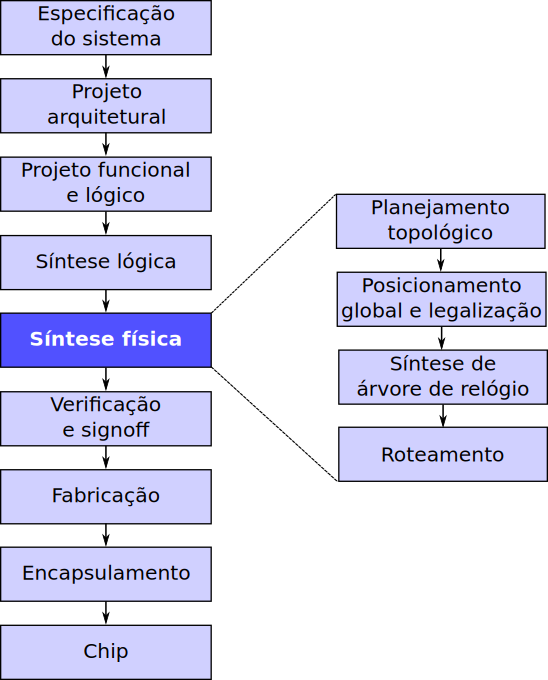
\includegraphics[width=0.5\textwidth]{img/introducao/exemplo_fluxo.pdf}
    \caption[Etapas do fluxo \textit{standard cell}.]{Exemplo das etapas de um fluxo de projeto com metodologia \textit{standard cell}. Figura adaptada de~\citeonline{kahng2011vlsi}.}
    \label{fig:exemplo_fluxo}
\end{figure}

Na etapa de síntese física as portas lógicas e os elementos sequenciais da \textit{netlist} são associados a descrições geométricas de associações de transistores referenciadas por "células", as quais estão disponíveis na \textit{standard cells}.
Após, as células são posicionadas e interconectadas, formando uma descrição completa das máscaras que serão usadas na fabricação do \ac{ic}.
Tal descrição ainda deve ser verificada antes de ser enviada para a fabricação (verificação e signoff).
A verificação é realizada seguindo regras que representam as limitações físicas do meio de fabricação.
Por exemplo, todos os fios devem estar a uma distância mínima e ter uma determinada largura mínima.
Uma vez fabricado, o \ac{ic} é testado e empacotado (etapa de encapsulamento).

Observe que a Figura~\ref{fig:exemplo_fluxo} apresenta um modelo simplificado do fluxo executado no projeto de um \ac{ic} real.
% Caso a Figura~\ref{fig:exemplo_fluxo} apresentasse o fluxo completo, seria necessário inserir diversas etapas de otimização, bem como caminhos que regressam no fluxo.
Note que este não é um fluxo linear, mas iterativo, onde pode ser necessário voltar para etapas anteriores do fluxo.
Por exemplo, caso ocorra um congestionamento numa determinada área do circuito, o roteamento do circuito pode se tornar impossível de ser realizado. Neste caso, o projeto deve retornar à etapa de posicionamento e legalização das células.

Ao mesmo tempo que cada etapa do fluxo \textit{standard cell} apresenta grande complexidade, segundo~\citeonline{papa2011physical}, é desejável que o fluxo completo de projeto seja realizado em um curto período de tempo (12 horas no processo da IBM). Logo, é essencial que cada etapa seja executada no menor tempo possível, o que demanda a exploração de diversas técnicas para redução de tempo de execução.
Portanto, as ferramentas de \ac{eda} devem tratar um grande volume de dados em um curto período de tempo.
Para isso, estas ferramentas devem empregar otimizações de software, como o uso de melhores estruturas de dados, paralelização e exploração da localidade de dados na cache.


% Diversos trabalhos na literatura buscam otimizar o tempo de execuções de aplicações.
% \citeonline{majeti2013compiler} utilizou heurísticas e metadados inseridos no código fonte para, em tempo de compilação, selecionar as estrutura de dados para execução em CPU\@/\@GPU.
% Já \citeonline{sung2010data} realizaram conversões das estruturas de dados para aumentar a utilização da cache compartilhada empregando transformações em tempo de compilação.
% Porém, a grande maioria destes trabalhos realizam as otimizações com foco em uma única arquitetura, avaliam seus resultados com \textit{benchmarks} sintéticos e nenhum destes trabalhos foi avaliado no contexto de \textit{Physical Design}.

% Outra adversidade que as ferramentas de \ac{eda} enfrentam é como modelar os dados para que as diversas relações do fluxo do projeto seja suportadas.
% Modelando com modelos tradicionais de programação, como \ac{ood}, a hierarquia das classes pode forçar a repetição de código e\@/\@ou a utilização de herança múltipla para um determinado problema.
% Herança múltipla não é suportada por todas as linguagens de programação e, mesmo quando suportada, não é recomendável porque pode levar a uma codificação confusa que dificultaria a manutenção do código~\cite{nystrom2014game}.

Este trabalho irá focar na exploração da localidade da cache no contexto de ferramentas de Physical Design.
Para aumentar a localidade da cache, este trabalho irá aplicar otimizações previamente ao código ser compilado.
Para realizar estas otimizações, primeiro serão identificadas as características de cada algoritmo e sobre quais dados este irá operar.
Posteriormente, será otimizada a organização destes dados de forma a maximizar a utilização dos dados recuperados pela cache.
Por fim, este trabalho ira comparar a abordagem tradicional (orientada a objetos) com a abordagem otimizada considerando o número total de \textit{cache misses} e o tempo de execução. Informações pertinentes a arquiteturas de cache (tamanho de blocos e número de níveis) não serão consideradas no momento da organização dos dados.
Estas informações não serão consideradas pois a organização dos dados deve suportar diversas arquiteturas de cache.


\section{Justificativa}

    Apesar de vários trabalhos encontrados na literatura fazerem otimizações de software mencionadas na seção anterior, nenhum deles avalia o impacto destas diferentes estratégias quando aplicadas no contexto de Physical Design.

    % Portanto, é desejável uma análise quantitativa do impacto da organização dos dados no contexto de Physical Design, sobretudo, com uma comparação que faça uso de uma infraestrutura realista e bem consolidada na academia.
    Portanto, é desejável uma análise quantitativa do impacto da organização dos dados no contexto de Physical Design, sobretudo, com um estudo de problemas reais utilizando entradas realistas para a experimentação.

\section{Objetivos e Contribuições Pretendidas}

    Este trabalho tem como objetivo a avaliação quantitativa do impacto causado pela organização dos dados em diferentes algoritmos no contexto de Physical Design.

    Os objetivos específicos deste trabalho são:

    \begin{itemize}
        \item Implementar três algoritmos de Physical Design com diferentes tipos de organização dos dados;
        \item Avaliar as organizações dos dados propostas comparando-as com a modelagem tradicional utilizada, resultante do uso de orientação a objetos. A comparação é realizada comparando o número de \textit{cache misses} gerados pelas algoritmos, bem como o tempo de execução;
        \item Avaliar a facilidade e o desempenho da paralelização dos algoritmos implementados com as diferentes organização dos dados.
    \end{itemize}

    Cumprindo estes objetivos, espera-se alcançar as seguintes contribuições científicas e tecnológicas:

    \begin{itemize}
        \item Implementação de um sistema de componentes e entidades;
        \item Avaliação quantitativa do desempenho causado pela modelagem dos dados em três algoritmos da síntese física;
        \item Resultados experimentais utilizando uma infraestrutura baseada em circuitos industriais;
        \item Resultados experimentais analisando problemas reais com dados realistas. Como dados de entrada serão utilizados circuitos industriais oriundos da competição ICCAD CAD Context 2015~\cite{kim2015}.
    \end{itemize}


% \section{Metodologia}
%         Implementar versões de problemas
%         avaliar quantitativamente o número de cache misses
%         avaliar quantitativamente o tempo de execução
%
% \section{Limitações(escopo) deste trabalho}
%         somente 3 problemas avaliados
%         somente uma arquitetura de processador e cache
%         paralelização com um chunk único

% \section{Organização deste trabalho}
\section{Organização deste texto}

O Capítulo~\ref{cap:trabalhos_correlatos} apresenta os trabalhos correlatos na otimização da organização dos dados para uma melhor utilização da cache.
No Capítulo~\ref{cap:tecnica_proposta} é apresentada a proposta de organização dos dados e os possíveis impactos causados pelas mesmas segundo o contexto de Physical Design.
O Capítulo~\ref{cap:resultados} apresenta os resultados preliminares já obtidos até o presente momento da escrita deste documento.
O Capítulo~\ref{cap:cronograma} descreve as atividades já realizadas e as que ainda precisam serem realizadas para a conclusão deste mestrado. Neste capítulo também é apresentado o cronograma que demonstra que este mestrado será concluído dentro do prazo disposto.

    % contextualização     do     problema;
    % objetivos;
    % metodologia;
    % contribuições;
% !TEX root = ../dissertacao.tex
\chapter{Trabalhos correlatos}
\label{cap:trabalhos_correlatos}

Este capítulo revisa os principais trabalhos de otimização do uso da memória cache.
Inicialmente, na Seção~\ref{sec:trabalhos_cache_aware} serão abordados os trabalhos correlatos que consideram informações da arquitetura da memória cache (\textit{cache-aware}).
Posteriormente, na Seção~\ref{sec:trabalhos_cache_oblivous} serão abordados os trabalhos que desprezam informações sobre a memória cache a qual o programa será executado (\textit{cache-oblivious}).
Por fim, na Seção~\ref{sec:analise_trabalhos_correlatos}, será apresentado um resumo do estado da arte e suas oportunidades de contribuições científicas.
É importante ressaltar que este capítulo não faz uma análise exaustiva de cada trabalho citado, mas busca apresentar as características mais relevantes das principais abordagens para otimização do uso da memória cache.

\section{Trabalhos correlatos considerando \textit{cache-aware}}
\label{sec:trabalhos_cache_aware}

Esta seção apresenta os trabalhos correlatos que consideram o modelo de \textit{cache-aware}.
Algoritmos \textit{cache-aware} são aqueles que possuem informações sobre a arquitetura da cache a priori.
Com estas informações estes trabalhos buscam otimizar seus comportamentos para extrair o máximo de desempenho de uma dada arquitetura.
Como por exemplo, uma multiplicação de matrizes pode ser realizada em blocos para melhorar a localidade da cache.

\begin{figure}[hb]
    \centering
    \subfigure[$1^a$ iteração]{\includegraphics[width=0.3\linewidth]{img/multiplicacao_matrix_a}}
    \subfigure[$2^a$ iteração]{\includegraphics[width=0.3\linewidth]{img/multiplicacao_matrix_b}}
    \subfigure[$3^a$ iteração]{\includegraphics[width=0.3\linewidth]{img/multiplicacao_matrix_c}}
    \caption[Exemplo multiplicação de matrizes]{Exemplo multiplicação de matrizes com abordagem tradicional.}
    \label{fig:multiplicacao_matriz}
\end{figure}

A Figura~\ref{fig:multiplicacao_matriz} apresenta como seria uma multiplicação de duas matrizes utilizando a abordagem tradicional. Nesta figura, os \textit{cache misses} são representados pelas setas e a linha pontilhada representa um \textit{cache hit}. Podemos notar que os blocos carregados para a cache não são reaproveitados no passo seguinte da multiplicação, o que irá gerar um grande aumento no numero de instruções executadas bem como no tempo toral de execução.

Um algoritmo \textit{cache aware} para a multiplicação de matrizes poderia tirar proveito do conhecimento do tamanho do bloco da cache para executar as operações em uma sub-matriz.
A multiplicação de matrizes em blocos é possível uma vez que esta operação é apenas uma enorme adição de uma pilha de produtos, não importando qual ordem estas adições são realizadas.
O único cuidado que se deve tomar neste caso é para que todos os produtos sejam realizados corretamente e contribuam para as somas adequadas.

\begin{figure}[hb]
    \centering
    \subfigure[$1^a$ iteração]{\includegraphics[width=0.3\linewidth]{img/multiplicacao_matrix_bloco_a}}
    \subfigure[$2^a$ iteração]{\includegraphics[width=0.3\linewidth]{img/multiplicacao_matrix_bloco_b}}
    \subfigure[$3^a$ iteração]{\includegraphics[width=0.3\linewidth]{img/multiplicacao_matrix_bloco_c}}
    \caption[Exemplo multiplicação de matrizes em blocos]{Exemplo multiplicação de matrizes em blocos.}
    \label{fig:multiplicacao_matriz_bloco}
\end{figure}

A Figura~\ref{fig:multiplicacao_matriz_bloco} ilustra a execução de um algoritmo \textit{cache aware} de multiplicação de matrizes. Por ter conhecimento do tamanho do bloco da cache em que este algoritmo será executado, são executadas operações de submatrizes de tamanho $4 \times 4$. Esta otimização faz com que o número de \textit{cache misses} seja reduzido drasticamente, uma vez que o bloco recuperado para a cache é totalmente utilizado.

% Um desses trabalhos tem como enfoque a modelagem da arquitetura perante um conjunto de aplicações.

% \subsection{\citeonline{DiazAlvarez2016}}

% O trabalho de \citeonline{DiazAlvarez2016} visa encontrar a melhor configuração de uma arquitetura cache para um conjunto pré definido de aplicações.
% O contexto deste trabalho inclui aplicações para dispositivos móveis e portanto, operados a bateria.
% Seu principal objetivo é reduzir o tempo de execução das aplicações, bem como, o consumo energético demandado pelas mesmas.
% Para determinar as arquiteturas, este trabalho visa encontrar a capacidade, tamanho do bloco e associatividade da cache.

% \citeonline{DiazAlvarez2016} tomaram como base o trabalho de \citeonline{wang2012dynamic}.
% \citeonline{wang2012dynamic} realizaram uma análise combinando análise estática e dinâmica para determinar as configurações da cache para sistemas embarcados de tempo real.
% Com isso, \citeonline{wang2012dynamic} minimizam o consumo de energia em até $74\%$.

% Para determinar as arquiteturas, \citeonline{DiazAlvarez2016} encontraram os parâmetros da cache baseados em \ac{ge}~\cite{dempsey2009foundations} utilizando \textit{tracers} e determinando a configuração baseado-se no tempo de execução e consumo de energia.
% Esta técnica garante uma redução no tempo de execução pois o algoritmo meta-heurístico converge mesmo com um curto número de gerações e tamanho da população; e a técnica adiciona um \textit{hash} para armazenar os valores objetivos de cada cache avaliada.
% Para avaliar o trabalho, foram utilizados os \textit{benchmarks} Mediabench~\cite{mediabench1997}.
% Esta técnica conseguiu reduzir o tempo de execução em $75\%$ em média, e obteve $96\%$ de redução de consumo de energia em média.

\subsection{\citeonline{majeti2013compiler}}

O trabalho de \citeonline{majeti2013compiler} possui como objetivo principal determinar o melhor \textit{layout} dos dados para um determinado programa. Segundo o autor, o \textit{layout} ideal para um programa computacional depende de se o mesmo é executado em um núcleo de CPU, uma GPU discreta, ou em uma GPU integrada (juntamente com outros fatores). Com isso, para obter programas que extraíssem todo o potencial de uma arquitetura, seria necessário rescrever o código fonte para cada arquitetura de CPU\@/\@GPU.

Para sanar o problema da reescrita do código para cada arquitetura, \citeonline{majeti2013compiler} propõem a inserção de metadados nos códigos-fonte. Estes metadados guiariam um compilador a selecionar as melhores estruturas de dados para uma dada arquitetura de CPU\@/\@GPU. Com isso, o compilador é capaz de escolher e converter os dados de \ac{aos} para \ac{soa} e vice versa.
% Neste trabalho também é apresentado que a escolha do \textit{layout} de dados que maximiza o número de acessos coalescidos (acessos que utilizam o mesmo bloco da cache e, portanto, minimizam o número de cache misses) em uma GPU é NP-completo~\cite{wu2013complexity}.
Majeti et al. ainda ressaltam que os metadados se fazem necessários pois a escolha de um leiaute de dados que maximiza o número de acessos coalescidos (acessos que utilizam o mesmo bloco da cache e, portanto, minimizam o número de cache misses) para uma GPU é NP-completo. A prova que esta escolha é da classe NP-completo foi realizada por~\citeonline{wu2013complexity}.


Para avaliar a eficiência da técnica de compilação proposta, os autores geraram \textit{benchmarks} sintéticos e avaliaram a execução compilando esses códigos com e sem os metadados. Em algumas arquiteturas como AMD 4-core A10-5880K CPU e NVIDIA Tesla M2050 GPU conseguiram um \textit{speedup}\footnote{A métrica \textit{speedup} representa a relação entre os tempos de execução da solução sequencial e a solução paralela para um determinado número de threads.} de até $27,11 \times$ e $29,50 \times$ respectivamente.

\section{Trabalhos correlatos considerando \textit{cache-oblivious}}
\label{sec:trabalhos_cache_oblivous}

Esta seção apresenta os trabalhos correlatos que consideram o modelo de \textit{cache-oblivious}.
Algoritmos \textit{cache-oblivious} (ou \textit{cache-tran\-scen\-dent}) são algoritmos projetados para explorar a memória cache de uma CPU sem ter o tamanho da mesma (ou o tamanho das linhas, etc.) como um parâmetro explícito~\cite{frigo1999cache}. Assim, um algoritmo \textit{cache-oblivious} é concebido para funcionar otimizadamente, sem modificação, em inúmeras arquiteturas com diferentes tamanhos de cache, ou para uma hierarquia de memória com diferentes níveis de cache e tamanhos variados.

\subsection{\citeonline{li2014}}

O trabalho de \citeonline{li2014} tem como enfoque o gerenciamento da cache compartilhada em processadores multi-core.
Segundo o autor, a gestão do compartilhamento de cache não é apenas para alcançar um bom desempenho, mas também para garantir um desempenho estável em um ambiente dinâmico; e considerando não apenas programas paralelos, mas também programas sequenciais co-executados uns com os outros.

Para identificar onde o gerenciamento da cache pode incidir, os autores descrevem um método para reorganizar o código para um \textit{layout} ideal com base no \ac{pdg}.
Com estas informações, é construído um \ac{trg}~\cite{gloy1999procedure} para otimizar o \textit{layout} do código em tempo de compilação.
A otimização realiza duas transformações: reordenamento global das funções e\@/\@ou reordenamento dos blocos inter-procedurais. Estes reordenamentos são baseados na afinidade do acesso à cache.

Para mensurar suas otimizações, os autores utilizaram os \textit{benchmarks} SPEC CPU 2006~\cite{spec2006}, realizando os experimentos tanto em uma máquina real como em um simulador de instruções da cache. Para medir a proporção de cache misses, utilizaram contadores de desempenho de hardware.
O método melhorou o desempenho de todos os programas em até $3\%$ quando estes foram executados separadamente (somente um programa por processador).
Quando executados mais de um programa por processador, este método obteve até $10,3\%$ de melhoria. Ao utilizar melhor a cache compartilhada, o método amplia a melhoria da transferência de \textit{hiper-threading} em $8\%$.

\subsection{\citeonline{Tang2015}}

O trabalho de \citeonline{Tang2015} visa preservar a localidade da cache em algoritmos de Programação Dinâmica no contexto de algoritmos cache-oblivious paralelos.
% Estes algoritmos geralmente aplicam estratégias de divisão e conquista recursivamente, o que assintoticamente atinge o uso ótimo da localidade temporal de uma cache sequencial.
Estes algoritmos geralmente subdividem o problema em instâncias menores, o que assintoticamente atinge o uso ótimo da localidade temporal de uma cache sequencial.
No entanto, o escalonamento das tarefas pela granularidade de suas dependências limita o paralelismo ao introduzir dependências artificiais entre subtarefas recursivas, além das decorrentes das equações de recorrência~\cite{Tang2015}.

Para realizar as otimizações, \citeonline{Tang2015} removeram as dependências artificiais. Com isso, foi possível agendar as tarefas prontas para execução assim que todas as restrições reais de dependência eram satisfeitas (instruções atômicas foram usadas para identificar e iniciar tarefas prontas). Assim, eles conseguiram preservar a otimização da cache herdada da estratégia de dividir e conquistar.
Com a paralelização e remoção das dependências artificiais, Tang et al. atingiram uma melhoria de 3 a 5 vezes no tempo absoluto de execução.

\subsection{\citeonline{qasem2017characterizing}}

% O trabalho de \citeonline{qasem2017characterizing} caracteriza o impacto no desempenho da organização dos dados em arquiteturas de \ac{hpc} com sistemas de memória heterogêneos e de vários níveis.

Segundo os autores, este é o primeiro trabalho a considerar a organização dos dados juntamente com o \textit{layout} da memória.
\citeonline{qasem2017characterizing} caracterizam os problemas de desempenho com a organização de dados em arquiteturas de memória heterogêneas, visando descobrir os cenários aos quais seria rentável realizar uma reorganização das estruturas de dados compartilhadas para uma maior performance.
Segundo o autor, a eficiência do acesso aos dados é impactada pelos padrões de acesso a memória, \textit{layout} da estrutura de dados e características do caminho sobre o qual os dados serão transferidos entre o processador e a unidade de memória.

Com base no estudo realizado sobre os efeitos das organização de dados tradicionais para sistemas de memória heterogêneos, como \ac{aos} e \ac{soa}, os autores propõem uma nova estrutura de dados denominada \ac{ca}.
Esta estrutura de dados se comporta tanto como \ac{aos} ou \ac{soa}, dependendo do tipo de acesso a dados que está sendo realizado.
As decisões sobre a organização dos dados considera três atributos principais: \textit{register pressure}, intensidade aritmética e esparsidade no acesso aos dados.

O estudo realizado por \citeonline{qasem2017characterizing} demonstrou que a abordagem de utilizar \ac{soa} nem sempre é lucrativa e que a escolha da organização dos dados deve considerar uma variedade de fatores, incluindo intensidade aritmética e esparsidade no acesso aos dados.
A nova estratégia de organização dos dados (\ac{ca}), que aborda as limitações das abordagens atuais (\ac{aos} e \ac{soa}), atingiu uma aceleração de uma ordem de magnitude em algumas arquiteturas.

\section{Análise qualitativa dos trabalhos correlatos}
\label{sec:analise_trabalhos_correlatos}

Esta seção apresenta uma análise dos trabalhos correlatos citados neste capítulo.
A Tabela~\ref{tab:resumo_trabalhos_correlatos} classifica os trabalhos correlatos de acordo com o modelo de memória cache utilizado (\textit{Cache-Aware} ou \textit{Cache-Oblivious}) e o momento em que a otimização ocorre.
Ela também identifica os casos de usos que foram utilizados em cada um dos trabalhos.


% Please add the following required packages to your document preamble:
% \usepackage{booktabs}
% \usepackage{lscape}
\begin{table}[hb]
\centering
\caption{Resumo dos trabalhos correlatos.}
\label{tab:resumo_trabalhos_correlatos}
\resizebox{\textwidth}{!}{%
\begin{tabular}{@{}cccc@{}}
\toprule
Trabalho      & Consideração da Cache & Momento da Otimização & Casos de Uso                                                               \\ \midrule
% Álvarez, 2016 & Cache-Aware           & N/A                   & Mediabench                                                                 \\
Majeti, 2013  & Cache-Aware           & Compilação            & sintéticos                                                                 \\
Li, 2014      & Cache-Oblivious       & Compilação            & SPEC2006 CPU                                                               \\
Tang, 2015    & Cache-Oblivious       & Pós-Compilação        & sintéticos                                                                 \\
Qasem, 2017   & Cache-Oblivious       & Pós-Compilação        & sintéticos                                                                 \\
Este Trabalho & Cache-Oblivious       & Pré-Compilação        & \begin{tabular}[c]{@{}c@{}}3 algoritmos de\\ Physical Design*\end{tabular} \\ \midrule
\multicolumn{4}{l}{* Entrada realista oriunda de circuitos industriais providos pela competição ICCAD2015 \cite{kim2015}.}                
\end{tabular}
}
\end{table}

Diversos métodos de otimizações já foram avaliados, dentre os quais se destacam:
heurísticas para selecionar estrutura de dados realizado por \citeonline{majeti2013compiler};
\citeonline{li2014} reorganizou as instruções baseando-se em grafo de dependências;
\citeonline{sung2010data} realizou conversão das estruturas de dados para aumentar a utilização da cache compartilhada empregando transformações em tempo de compilação.
Porém, a grande maioria destes trabalhos avaliam seus resultados com \textit{benchmarks} sintéticos e nenhum destes trabalhos considera o contexto de \textit{Physical Design}.

Não foram localizados trabalhos que considerassem otimizações de software para \textit{cache-oblivious} no contexto de \textit{Physical Design}.
Portanto este trabalho possui como principal diferencial a aplicação de técnicas de otimizações no contexto de \textit{Physical Design}.
Estas otimizações serão implementadas numa biblioteca open-source para ensino e pesquisa de síntese física chamada Ophidian~\cite{ophidian}.
Este trabalho aborda o modelo de \textit{Cache-Oblivious} por ser uma biblioteca open-source e as otimizações carecem suportar diversas arquiteturas.
Para avaliar os 3 algoritmos de \textit{Physical Design} considerando um senário realista, este trabalho irá utilizar circuitos industriais providos para a análise do problema C da competição ICCAD 2015 CAD Contest~\cite{kim2015}.

    % revisão bibliográfica;
 \chapter{Técnica Proposta}
\label{cap:tecnica_proposta}

% Este capítulo apresenta a técnica proposta para resolver o problema de legalização incremental formulado na Seção \ref{sec:formulacao_incremental}, a qual adapta o algoritmo de \citeonline{chow2014cell} para utilizar uma estrutura de dados especializada no armazenamento de dados geométricos chamada R-tree. Inicialmente, este capítulo descreve, por meio de um exemplo, o processo de legalização incremental. Em seguida, apresenta como a R-tree realiza operações espaciais de forma rápida, para enfim apresentar os detalhes da adaptação proposta.

% \section{Processo de legalização incremental}

apresentar modelo de memoria
apresentar como cache miss funciona
apresentar ood
apresentar limitação do ood
apresentar dod
apresentar entity system
Discutir como o DOD reduz o numero de cache misses
como aplicar o dod em problemas
    Problema A - limites do chip
        como seria modelado OOD
        como seria modelado DOD
    Problema B - interconexão
        como seria modelado OOD
        como seria modelado DOD
    Problema C - cluster
        como seria modelado OOD
        como seria modelado DOD
    % proposta;
% !TEX root = ../dissertacao.tex
\chapter{Resultados Experimentais Preliminares}
\label{cap:resultados}

Este capítulo apresenta os resultados experimentais preliminares obtidos por este trabalho até o momento da escrita deste documento. Inicialmente, ele descreve a infraestrutura experimental utilizada. Em seguida, analisa três algoritmos de Physical Design. Por fim, apresenta uma síntese dos resultados e apresenta algumas melhorias e expectativas dos trabalhos a serem realizados até o a conclusão do mestrado.

\section{Infraestrutura experimental}
\label{sec:infraestrutura_experimental}

Os experimentos realizados utilizaram o conjunto de benchmarks disponibilizados pela competição \textit{ICCAD 2015 CAD Contest (problema C: Incremental Timing-Driven Placement)} \cite{kim2015}, o qual inclui 8 circuitos que possuem entre 768k e 1,93M células, todos derivados de circuitos industriais. Optou-se por utilizar tal infraestrutura pois a mesma disponibiliza circuitos com número de células compatível com circuitos contemporâneos. Além disso, tal infraestrutura é de acesso aberto, o que facilita a comparação experimental deste trabalho com futuros trabalhos que possivelmente serão realizados por terceiros. Como biblioteca básica, utilizou-se a Ophidian: Open-Source Library for Physical Design Research and Teaching~\cite{ophidian}.

Todos os experimentos foram executados em um computador Linux com processador Intel\textsuperscript{\textregistered} Core\textsuperscript{\textregistered} i5-4460 CPU @ 3.20~GHz.
A Figura~\ref{fig:architectureMemoryZeus} apresenta de forma gráfica a arquitetura deste computador.
Este computador possui 32GB~RAM (DDR3 a 1600MHz) como memória principal.
Seu processador possui quatro núcleos idênticos e três níveis de cache.
Os primeiros dois níveis de cache~(L1 and L2) são privados para cada core do processador e possuem 64KB e 256KB de capacidade respectivamente.
O terceiro nível da cache~(L3) é compartilhado entre todo o processador e possui 6144KB de capacidade.

\begin{figure}[ht]
    \centering
    \includegraphics[width=0.5\linewidth]{img/results/architectureMemoryZeus.pdf}
    \caption{Arquitetura do computador utilizados nos experimentos.}
    \label{fig:architectureMemoryZeus}
\end{figure}

Os experimentos que avaliam o tempo de execução podem apresentar resultados diferentes em cada realização, devido a variações causadas pelo computador utilizado. Portanto, para aumentar a confiança estatística obtida pelos experimentos, os mesmos foram repetidos 30 vezes.% , o que resultou em 99\% de confiança estatística\footnote{A confiança estatística foi medida utilizando o teste t de Student para p=0,01.}.

\section{Metodologia Experimental}
\label{sec:metodologia_experimental}

Para avaliar o impacto que a organização dos dados pode causar em problemas de \textit{Physical Design}, será avaliado o \textbf{número de cache misses} e o \textbf{tempo de execução} para três algoritmos. São eles:
\begin{itemize}
    \item Problema A: Verificar se cada célula do circuito está contida dentro dos  limites físicos do circuito integrado. Neste cenário somente uma propriedade é necessário para cada célula. Portanto, a localidade dos dados será totalmente explorada na implementação com \ac{dod}. Sendo assim, este problema representa o melhor caso para implementações com o modelo de dados \ac{dod};
    \item Problema B: Estimar o comprimento de todas as interconexões do circuito. Este cenário acessa diferentes propriedades de diferentes entidades. Portanto, não pode explorar eficientemente a localidade de dados fornecida por \ac {dod}, uma vez que as propriedades dos pinos em uma única interconexão podem não ser contíguas na memória, a menos que a matriz de propriedades esteja previamente agrupada;
    \item Problema C: Clusterização de Registradores. Este cenário representa uma tarefa mais complexa que pertence a síntese física de um \ac{ic}.
\end{itemize}

Para cada problema listado acima, foram implementados protótipos de software seguindo duas organizações de dados: \ac{ood} e \ac{dod}.
Estes protótipos foram implementados utilizando linguagem de alto nível C++ e o código fonte encontra-se disponível online no repositório GitHub da Ophidian~\cite{ophidian}.

As Subseções \ref{sec:problema_a} a \ref{sec:problema_c} a seguir apresentam os resultados preliminares para os três algoritmos avaliados.
Para uma maior confiança estatística, todos os resultados apresentados nestas seções são a média de 30 execuções.
Por fim, a Subseção \ref{sec:sintese_resultado} apresenta uma síntese de todos os resultados.

\section{Estudo de Caso A:}
\label{sec:problema_a}

A Figura \ref{fig:missProblemA} apresenta o número de cache misses (eixo Y) em milhões para cada circuito avaliado (eixo X). As barras vermelhas representam o modelo de dados Orientado a Objetos (\ac{ood}). As barras azuis representam o modelo Orientado a Dados (\ac{dod}). O número total de cache misses para o \ac{dod} (de $0,5M$ a $1,4M$) foi, em média, um décimo do número atingido pelo modelo \ac{ood} (de $5,4M$ a $13,7M$). A redução no número de cache misses é proveniente diretamente da melhor organização dos dados em memória. Nesta organização, os dados de uma mesma propriedade (posição de uma determinada célula neste problema) estão armazenados contiguamente em memória. Portanto, ao ocorrer um miss na cache, somente dados úteis são recuperados da memória principal. Assim, é realizado um melhor aproveitamento dos blocos de dados recuperados da memória principal para a cache.

\begin{figure}[ht]
    \centering
    \includegraphics[width=0.65\linewidth]{img/results/missProblemA}
    \caption[Cache misses do Problema~A.]{Número de cache misses resultantes dos dois protótipos de software do Problema~A.}
    \label{fig:missProblemA}
\end{figure}

A exploração da localidade de dados reduz o tempo de acesso à memória principal, que representa o gargalo principal. Esta redução no tempo de acesso a memória pode ser observada na Figura~\ref{fig:runtimeProblemA}. Este gráfico retrata o tempo de execução (eixo Y) em milissegundos para cada circuito avaliado (eixo X). Pode-se observar que a versão \ac{dod} executou mais rápido em todos os circuitos avaliados. Os tempos de execução da versão \ac{dod} foram entre $4ms$ e $12ms$, enquanto os tempos de execução de \ac{ood} foram entre $74ms$ e $186ms$. Portanto, para o problema~A, \ac{dod} é em média $94\%$ ($16\times$) mais rápido do que \ac{ood}.

\begin{figure}[ht]
    \centering
    \includegraphics[width=0.65\linewidth]{img/results/runtimeProblemA}
    \caption[Tempo de execução Problema~A]{Tempo de execução para o Problema~A.}
    \label{fig:runtimeProblemA}
\end{figure}

\section{Estudo de Caso B:}
\label{sec:problema_b}

Com objetivo de avaliar o impacto da organização dos dados no pior cenário para o \ac{dod}. Nesta etapa do trabalho foi avaliado uma tarefa que necessite de diversas propriedades para solucionar o problema.
Diferente do Estudo de Caso~A, nesta tarefa é necessário acessar diferentes \textit{entity-component systems} (interconexões e pinos) e múltiplas propriedades. Complementarmente, os pinos pertencentes a cada interconexão podem não estar contíguos em memória, o que impacta na performance.

A Figura~\ref{fig:runtimeProblemB} apresenta o número de cache misses resultantes para cada modelo de programação. Pode-se observar que o número de cache misses do \ac{dod} (de $253M$ a $819M$) foi, em média, $10\%$ maior do que quando comparado ao modelo \ac{ood} (de $231M$ a $749M$). O maior número de cache misses do \ac{dod} resultou em uma performance inferior para o Problema~B. Contudo, o modelo \ac{dod} ainda proporcionou uma melhor engenharia de software. Adicionalmente, a diferença de performance no Problema~B (quando o \ac{dod} é mais lento) é muito menor do que a performance atingida no Problema~A (quando o \ac{dod} é mais rápido).

\begin{figure}[ht]
    \centering
    \includegraphics[width=0.7\linewidth]{img/results/missProblemB}
    \caption[Cache misses do Problema~B.]{Número de cache misses resultantes dos dois protótipos de software do Problema~B.}
    \label{fig:missProblemB}
\end{figure}

Na Figura~\ref{fig:runtimeProblemB} esta apresentado o tempo de execução (eixo Y) em milissegundos para cada circuito avaliado (eixo X). O tempo de execução para o \ac{dod} foi entre $3497ms$ e $10300ms$, enquanto o tempo de execução do \ac{ood} foi $3306ms$ e $9654ms$. Como consequência do maior número de cache misses, no Problema~B o modelo \ac{ood} foi em média $6\%$ mais rápido do que o modelo \ac{dod}.

\begin{figure}[ht]
    \centering
    \includegraphics[width=0.7\linewidth]{img/results/runtimeProblemB}
    \caption[Tempo de execução Problema~B]{Tempo de execução para o Problema~B.}
    \label{fig:runtimeProblemB}
\end{figure}

\section{Estudo de Caso C:}
\label{sec:problema_c}

A Clusterização de Registradores consiste em identificar células síncronas próximas e agrupá-las em um único \textit{cluster}. Para resolver este problema foi implementado o algoritmo clássico K-Means~\cite{selim1984k}. K-Means é um algoritmo clássico de agrupamento de elementos, não utilizado somente para register clustering, mas também em diferentes áreas como: \textit{machine learning} e \textit{data mining}.

Para avaliar como a organização dos dados pode impactar no desempenho desta tarefa, foram implementados duas versões (sequencial e paralela) para cada modelo de organização dos dados (\ac{ood} e \ac{dod}).
A Subseção~\ref{subsec:execucaoSequencialProblemaC} irá discutir os resultados preliminares para a execução sequencial, ao passo que, a Subseção~\ref{subsec:execucaoParalelaProblemaC} ira abordar os resultados da execução paralela.

\subsection{Execução Sequencial}
\label{subsec:execucaoSequencialProblemaC}

A Figura~\ref{fig:missProblemC_sequential_rtree} apresenta o número total de cache misses (eixo Y) em milhões para cada circuito avaliado (eixo X).
O número de cache misses para a Orientação a Dados (\ac{dod}) (de $17M$ a $173M$) foi, em média, $24\%$ menor do que o número requerido pela Orientação a Objetos (\ac{ood}) (de $29M$ a $214M$).
Este resultado indica, como o esperado, que a localidade espacial foi melhor utilizada quando aplicou-se o \ac{dod}.

\begin{figure}[ht]
    \centering
    \includegraphics[width=0.7\linewidth]{img/results/missProblemC_sequential_rtree}
    \caption[Cache misses Problema~C versão sequencial]{Número de cache misses para a implementação sequencial da Clusterização de Registradores}
    \label{fig:missProblemC_sequential_rtree}
\end{figure}

O menor número de cache misses com \ac{dod} impactou no tempo de execução para esta tarefa.
A Figura~\ref{fig:runtimeProblemC_sequential_rtree} apresenta a média dos tempos de execuções (eixo Y) em milissegundos para cada circuito avaliado (eixo X).
O tempo necessário para o \ac{dod} concluir a tarefa foi entre $724ms$ e $2364ms$, enquanto quando utilizado o \ac{ood} foi entre $804ms$ e $2526ms$.
Em média, o \ac{dod} executou $7,5\%$ mais rápido que o \ac{ood}.
Portanto, estes resultados confirmam que uma melhor organização dos dados em memória podem impactar beneficamente no tempo de execução de tarefas de \textit{Physical Design}.

Pode-se notar também que a redução no número de cache misses não impactou na mesma proporção no tempo de execução. Isto se deve ao fato de que a organização dos dados impactou somente em instruções de acesso a dados em memória, sendo este conjunto um subconjunto de todas as instruções do software.

\begin{figure}[ht]
    \centering
    \includegraphics[width=0.7\linewidth]{img/results/runtimeProblemC_sequential_rtree}
    \caption[Tempo de execução Problema~C versão sequencial]{Tempo de execução para a implementação sequencial da Clusterização de Registradores}
    \label{fig:runtimeProblemC_sequential_rtree}
\end{figure}

\subsection{Execução Paralela}
\label{subsec:execucaoParalelaProblemaC}

Com objetivo de avaliar o comportamento das estruturas de dados em ambientes paralelos, foi implementado uma versão paralela do algoritmo K-Means.
A Figura~\ref{fig:missProblemC_parallel_rtree} apresenta o número total de cache misses (eixo Y) em milhões para cada circuito avaliado (eixo X) na implementação paralela.
Pode-se notar que o número total de cache misses reduziu comparado as versões sequenciais. Isto se deve ao fato de que a implementação paralela usa os caches L1 e L2 de todos os núcleos, aumentando a quantidade de memória disponível. Outro benefício é que o terceiro nível da cache (L3) é compartilhado entre todos os cores do processador.
O número de falhas na cache para \ac{dod} (de $7M$ a $131M$) foi, em média, $20\%$ menor do que o alcançado pelo \ac{ood} (de $17M$ a $159M$). Este resultado demonstra que, como esperado, a organização de dados levou a um número menor de cache misses, mesmo para a implementação paralela.

\begin{figure}[ht]
    \centering
    \includegraphics[width=0.7\linewidth]{img/results/missProblemC_parallel_rtree}
    \caption[Cache misses Problema~C versão paralela]{Número de cache misses para a implementação paralela de Clusterização de Registradores}
    \label{fig:missProblemC_parallel_rtree}
\end{figure}

A redução de cache misses impactou novamente no tempo de execução. A Figura~\ref{fig:runtimeProblemC_parallel_rtree} mostra os resultados de tempo de execução (eixo Y) em milissegundos para a implementação paralela. Os tempos de execução do \ac{dod} foram entre $264ms$ e $769ms$, enquanto que os tempos de execução da implementação que utilizou \ac{ood} foram entre $ 300ms $ e $ 896ms $. Portanto, o modelo de programação \ac{dod} é, em média, $ 15.5\% $ mais rápido que o modelo \ac{ood} quando ambos são paralelizados.


\begin{figure}[ht]
    \centering
    \includegraphics[width=0.7\linewidth]{img/results/runtimeProblemC_parallel_rtree}
    \caption[Tempo de execução Problema~C versão paralela]{Tempo de execução para a implementação paralela da Clusterização de Registradores}
    \label{fig:runtimeProblemC_parallel_rtree}
\end{figure}

Observe que, enquanto a implementação sequencial \ac{dod} é em média $ 7.5 \% $ mais rápida do que a implementação \ac{ood}, na implementação paralela essa diferença aumentam para $ 15 \% $.
Esses resultados mostram que a aceleração alcançada pela implementação paralela é maior quando aplicada usando o modelo de programação \ac{dod}, mesmo que a diferença no número de cache misses seja menor entre as implementações ($ 20 \% $ no cenário paralelo comparado a $ 24 \% $ no cenário sequencial).

Na verdade, considerando apenas as versões orientadas a dados (\ac{dod}), a implementação paralela alcançou um speedup médio de $ 3,04 $ em relação a implementação sequencial, enquanto ao comparar as duas versões  orientadas a objetos (\ac{ood}) speedup foi de apenas $ 2,78 $.
Um possível motivo para esses resultados pode advir de que o tempo de acesso à memória seja um fator mais relevante nas implementações paralelas do que nas sequenciais, tornando a programação com \ac{dod} ainda mais eficiente neste cenário.


\section{Síntese dos Resultados e Perspectivas}
\label{sec:sintese_resultado}

Nesta Seção será apresentados brevemente uma síntese dos resultados preliminares obtidos até a escrita deste documento. Posteriormente serão apresentadas as perspectivas de melhorias destes resultados.

A Tabela~\ref{tab:sintese_resultados} apresenta um breve resumo das reduções/acréscimos médios da técnica \ac{dod} sobre a técnica \ac{ood} no número de cache misses e tempo de execução.
Nesta tabela, números negativos em cache misses significam que a técnica \ac{dod} resultou em menor número de cache misses.
Ao passo que, números negativos no tempo de execução representam que a técnica \ac{dod} executou mais rápido que a técnica \ac{ood}.

É possível identificar, tendo como base a Tabela~\ref{tab:sintese_resultados}, de que existem classes de problemas cujo o modelo de programação \ac{dod} pode superar em até dezesseis vezes ($16 \times$) o modelo de programação \ac{ood}.
Porém, no caso em que o modelo \ac{dod} foi inferior no desempenho, a modularidade e a engenharia de software continuaram sendo superiores às que foram implementadas seguindo o modelo \ac{ood}.


\begin{table}[h]
\centering
\caption{Síntese dos resultados preliminares.}
\label{tab:sintese_resultados}
\resizebox{\textwidth}{!}{
\begin{tabular}{c|r|r|r|r|}
\cline{2-5}
                                 & \multicolumn{2}{c|}{Execução Sequencial}                                               & \multicolumn{2}{c|}{Execução Paralela}                                                 \\ \cline{2-5}
                                 & \multicolumn{1}{c|}{\# Cache misses} & \multicolumn{1}{c|}{Tempo de Execução} & \multicolumn{1}{c|}{\# Cache misses} & \multicolumn{1}{c|}{Tempo de Execução} \\ \hline
\multicolumn{1}{|c|}{Problema A} & - 90\%                              & - 94\%                                & ---                                     & ---                                   \\ \hline
\multicolumn{1}{|c|}{Problema B} & + 10\%                              & + 6\%                                 &  ---                                    & ---                                   \\ \hline
\multicolumn{1}{|c|}{Problema C} & - 24\%                              & - 7.5\%                               & - 20\%                                  & - 15.5\%                              \\ \hline
\end{tabular}
}
\end{table}

Como perspectivas para melhorar ainda mais a organização dos dados, pretende-se implementar um modelo de \textit{entity-component system} que suporte o agrupamento das propriedades de uma entidade.
Suportar o agrupamento das propriedades possivelmente irá melhorar o desempenho das implementações.
Uma vez que, em determinadas tarefas é importante acessar os dados numa dada ordem.

Na Figura~\ref{fig:sorting_data_example}~(a) pode-se observar o mapeamento da estimativa de comprimento das interconexões (Problema B), utilizando a técnica \ac{dod}, sem nenhum agrupamento nos dados.
Para determinar o comprimento de uma interconexão (\textit{Net}), seguindo o modelo de interconexão \ac{hpwl}\footnote{O modelo de interconexão \ac{hpwl} é calculado como a metade do perímetro mínimo de todos os pinos de uma interconexão.}, é necessário determinar o perímetro mínimo que abrange todos os pinos.
Para isso, é necessário acessar todas as posições dos pinos pertencentes a esta interconexão.
Seguindo o exemplo da~\ref{fig:sorting_data_example}~(a) e supondo que iremos calcular o \ac{hpwl} da interconexão $N1$, cujo índice é $0$, podemos notar que os pinos pertencentes a $N1$ não estão contíguos na memória.
Esta esparsidade nos dados pode depreciar o desempenho do acesso aos dados e exigir um número maior de \textit{cache misses} para a recuperação de todos os dados requeridos pelo algoritmo.

Para evitar este efeito de acesso não continuo na memória, é desejável possuir os dados agrupados segundo uma determinada característica, como por exemplo os pinos pertencentes a uma mesma interconexão. A Figura~\ref{fig:sorting_data_example}~(b) apresenta um possível agrupamento dos dados em relação a cada interconexão.
Este agrupamento possivelmente reduz o número de falhas na cache pois cada bloco recuperado pelo \textit{cache miss} seria melhor aproveitado.


\begin{figure}[t]
    \centering
    \subfigure[Dados sem agrupamento]{\includegraphics[width=\linewidth]{img/results/sorting_data_example_original}}

    \subfigure[Dados agrupados pelas interconexões]{\includegraphics[width=\linewidth]{img/results/sorting_data_example_grouping}}
    \caption[Exemplo de agrupamento dos dados]{Exemplo de possível agrupamento nos dados para problema de estimativa do comprimento de interconexão. Cada propriedade está contiguamente armazenada em memória. (a) representa as propriedades sem nenhum agrupamento de dados. (b) representa os mesmos dados apresentados em (a) porém, com as interconexões propriedades agrupadas pelas interconexões.}
    \label{fig:sorting_data_example}
\end{figure}



\chapter{Cronograma}
\label{cap:cronograma}

Este capítulo apresenta as atividades já concluídas até o momento da escrita deste documento, assim como as atividades pendentes que serão realizadas após o exame de qualificação.

\section{Atividades concluídas}

\begin{itemize}
    \item \textbf{C1}: Implementar problemas de \textit{Physical Design} utilizando \ac{ood} e \ac{dod}.
    \item \textbf{C2}: Avaliar quantitativamente os resultados obtidos na Atividade C1.
    \item \textbf{C3}: Escrita e submissão do artigo para o ISPD 2017 (Qualis A2).
    \item \textbf{C4}: Implementar técnica de clusterização de elementos utilizando \ac{ood} e \ac{dod}.
    \item \textbf{C5}: Avaliar quantitativamente os resultados obtidos na Atividade C4.
    \item \textbf{C6}: Escrita e submissão do artigo para o SBCCI 2017 (Qualis B1).
    \item \textbf{C7}: Apresentação do artigo no SBCCI 2017.
    \item \textbf{C8}: Escrita do texto do Exame de Qualificação.
    % \item \textbf{C9}:
    % \item \textbf{C10}:
\end{itemize}

\section{Atividades pendentes}

\begin{itemize}
    \item \textbf{P1}: Realizar as sugestões de melhoria do trabalho propostas pela banca no exame de qualificação;
    \item \textbf{P2}: Implementar Sistema de Entidade com suporte a acesso ordenado das propriedades de uma entidade.
    \item \textbf{P3}: Adaptar problemas já implementados nas atividades C1 e C4 para ordenarem as propriedades pela ordem de acesso.
    \item \textbf{P4}: Avaliar quantitativamente os resultados obtidos na Atividade P3.
    \item \textbf{P5}: Escrever e submeter artigo para revista ou evento de índice restrito com as contribuições totais deste trabalho.
    \item \textbf{P6}: Escrever a dissertação de mestrado;
    \item \textbf{P7}: Preparar a apresentação e defender este trabalho de mestrado;
    \item \textbf{P8}: Realizar as correções sugeridas pela banca durante a defesa;
    \item \textbf{P9}: Entregar a versão final da dissertação de mestrado na Biblioteca Central da Universidade Federal de Santa Catarina.
\end{itemize}

\section{Cronograma}

A Figura~\ref{tab:cronograma} apresenta o cronograma o previsto para realização deste trabalho de mestrado.
Os meses de Novembro e Dezembro serão dedicados às correções sugeridas pela banca no exame de qualificação, assim como a implementação do ordenamento no sistema de entidades.
Finalizando as correções, entre Janeiro e Março pretende-se terminar toda a análise experimental o que suportará a escrita de um artigo, que será realizado nos meses de Março e Abril.
Por fim, os meses entre Maio e Julho são reservados para realizar as correções sugeridas pela banca na defesa e entrega do artigo na Biblioteca Central da Universidade Federal de Santa Catarina.
Desta forma, a finalização deste trabalho de mestrado está dentro do prazo de 24 meses previsto pelo programa de Pós-Graduação em Ciência da Computação da Universidade Federal de Santa Catarina.


\begin{table}[b]
\centering
\caption[Cronograma do trabalho]{Cronograma previsto para realização do trabalho de mestrado}
\label{tab:cronograma}
\resizebox{\textwidth}{!}{
\begin{tabular}{@{}cccccccccc@{}}
\toprule
                                  & \textbf{Novembro}      & \textbf{Dezembro}      & \textbf{Janeiro}       & \textbf{Fevereiro}     & \textbf{Março}         & \textbf{Abril}         & \textbf{Maio}          & \textbf{Junho}         & \textbf{Julho}         \\ \midrule
\multicolumn{1}{|c|}{\textbf{P1}} & \multicolumn{1}{c|}{X} & \multicolumn{1}{c|}{}  & \multicolumn{1}{c|}{}  & \multicolumn{1}{c|}{}  & \multicolumn{1}{c|}{}  & \multicolumn{1}{c|}{}  & \multicolumn{1}{c|}{}  & \multicolumn{1}{c|}{}  & \multicolumn{1}{c|}{}  \\ \midrule
\multicolumn{1}{|c|}{\textbf{P2}} & \multicolumn{1}{c|}{}  & \multicolumn{1}{c|}{X} & \multicolumn{1}{c|}{X} & \multicolumn{1}{c|}{}  & \multicolumn{1}{c|}{}  & \multicolumn{1}{c|}{}  & \multicolumn{1}{c|}{}  & \multicolumn{1}{c|}{}  & \multicolumn{1}{c|}{}  \\ \midrule
\multicolumn{1}{|c|}{\textbf{P3}} & \multicolumn{1}{c|}{}  & \multicolumn{1}{c|}{X} & \multicolumn{1}{c|}{X} & \multicolumn{1}{c|}{X} & \multicolumn{1}{c|}{}  & \multicolumn{1}{c|}{}  & \multicolumn{1}{c|}{}  & \multicolumn{1}{c|}{}  & \multicolumn{1}{c|}{}  \\ \midrule
\multicolumn{1}{|c|}{\textbf{P4}} & \multicolumn{1}{c|}{}  & \multicolumn{1}{c|}{X} & \multicolumn{1}{c|}{X} & \multicolumn{1}{c|}{X} & \multicolumn{1}{c|}{}  & \multicolumn{1}{c|}{}  & \multicolumn{1}{c|}{}  & \multicolumn{1}{c|}{}  & \multicolumn{1}{c|}{}  \\ \midrule
\multicolumn{1}{|c|}{\textbf{P5}} & \multicolumn{1}{c|}{}  & \multicolumn{1}{c|}{}  & \multicolumn{1}{c|}{}  & \multicolumn{1}{c|}{}  & \multicolumn{1}{c|}{X} & \multicolumn{1}{c|}{X} & \multicolumn{1}{c|}{}  & \multicolumn{1}{c|}{}  & \multicolumn{1}{c|}{}  \\ \midrule
\multicolumn{1}{|c|}{\textbf{P6}} & \multicolumn{1}{c|}{X} & \multicolumn{1}{c|}{X} & \multicolumn{1}{c|}{X} & \multicolumn{1}{c|}{X} & \multicolumn{1}{c|}{X} & \multicolumn{1}{c|}{X} & \multicolumn{1}{c|}{X} & \multicolumn{1}{c|}{}  & \multicolumn{1}{c|}{}  \\ \midrule
\multicolumn{1}{|c|}{\textbf{P7}} & \multicolumn{1}{c|}{}  & \multicolumn{1}{c|}{}  & \multicolumn{1}{c|}{}  & \multicolumn{1}{c|}{}  & \multicolumn{1}{c|}{}  & \multicolumn{1}{c|}{}  & \multicolumn{1}{c|}{X} & \multicolumn{1}{c|}{X} & \multicolumn{1}{c|}{}  \\ \midrule
\multicolumn{1}{|c|}{\textbf{P8}} & \multicolumn{1}{c|}{}  & \multicolumn{1}{c|}{}  & \multicolumn{1}{c|}{}  & \multicolumn{1}{c|}{}  & \multicolumn{1}{c|}{}  & \multicolumn{1}{c|}{}  & \multicolumn{1}{c|}{}  & \multicolumn{1}{c|}{X} & \multicolumn{1}{c|}{X} \\ \midrule
\multicolumn{1}{|c|}{\textbf{P9}} & \multicolumn{1}{c|}{}  & \multicolumn{1}{c|}{}  & \multicolumn{1}{c|}{}  & \multicolumn{1}{c|}{}  & \multicolumn{1}{c|}{}  & \multicolumn{1}{c|}{}  & \multicolumn{1}{c|}{}  & \multicolumn{1}{c|}{}  & \multicolumn{1}{c|}{X} \\ \bottomrule
\end{tabular}
}
\end{table}
% 

    % cronograma de desenvolvimento das atividades previstas, incluindo provável mês e ano da defesa;



% % !TEX root = ../dissertacao.tex
\chapter{Introdução}
\label{cap:introducao}
    % evolução da tecnologia -> transistores menores
    % circuitos modernos muito grande grandes -> ferramentas de EDA
    % eletrônica de consumo -> tempo limitado para projeto de um circuito
    % é benéfico a redução de tempo na execução dos algoritmos sem perda da qualidade da solução
    % memória representa gargalo -> explorar a localidade na cache
    %
    % uma possível solução que não altera a qualidade da solução é o melhor armazenamento dos dados

A evolução da tecnologia de fabricação de \acp{ic} vem permitindo uma redução drástica e contínua das dimensões dos transistores.
O consequente aumento de densidade permitiu que atualmente sejam fabricados \acp{ic} com dezenas de milhões de transistores.
Além deste número elevado de elementos, os circuitos contemporâneos devem respeitar uma ampla gama de restrições, sejam elas de atraso, potência e\@/\@ou área.
Adicionalmente, o prazo entre o projeto e a fabricação de um chip é cada vez mais limitado para que um novo produto eletrônico possa garantir o mercado (\textit{time-to-market})~\cite{papa2011physical}.
Neste contexto, é mandatório o uso de Ferramentas de \ac{eda} no projeto de \acp{ic} contemporâneos.
% Portanto, as Ferramentas de \ac{eda} são obrigatórias no design de \acp{ic} modernos.

% Ferramentas de \ac{eda} para o projeto de circuitos digitais seguem uma metodologia de projeto denominada \textit{standard cell}.
O fluxo de projeto com ferramentas de \ac{eda} segue a metodologia denominada \textit{standard cell}.
Esta metodologia se caracteriza pela adoção de bibliotecas de células padrão pré-projetadas e pré-caracterizadas, que descrevem as informações lógicas, físicas e elétricas dos elementos combinacionais e sequenciais a serem utilizados na síntese~\cite{kahng2011vlsi}.

Um fluxo de projeto que segue a metodologia \textit{standard cell} é tipicamente dividido em diversas etapas.
A Figura~\ref{fig:exemplo_fluxo} apresenta as principais etapas deste fluxo, onde cada etapa pode ser subdividida em outras.
Este fluxo inicia com a captura do comportamento do sistema, em um alto nível de abstração (especificação do sistema).
Após, o sistema é particionado em \textit{software} e \textit{hardware} e a arquitetura da parte de \textit{hardware} é definida (projeto arquitetural).
A seguir, é criada a descrição no \ac{rtl}, usando uma \ac{hdl}, tal como VHDL e Verilog (projeto funcional e lógico).
Tal descrição é traduzida para o nível lógico (síntese lógica), originando uma lista de portas lógicas, elementos sequenciais (\textit{latches} e\@/\@ou \textit{flip-flops}) e interconexões, geralmente referenciada por \textit{netlist}.

\begin{figure}[]
    \centering
    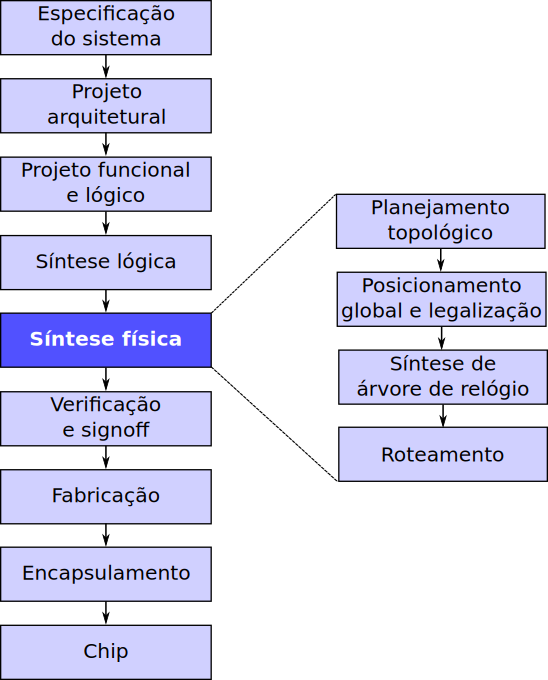
\includegraphics[width=0.5\textwidth]{img/introducao/exemplo_fluxo.pdf}
    \caption[Etapas do fluxo \textit{standard cell}.]{Exemplo das etapas de um fluxo de projeto com metodologia \textit{standard cell}. Figura adaptada de~\citeonline{kahng2011vlsi}.}
    \label{fig:exemplo_fluxo}
\end{figure}

Na etapa de síntese física as portas lógicas e os elementos sequenciais da \textit{netlist} são associados a descrições geométricas de associações de transistores referenciadas por "células", as quais estão disponíveis na \textit{standard cells}.
Após, as células são posicionadas e interconectadas, formando uma descrição completa das máscaras que serão usadas na fabricação do \ac{ic}.
Tal descrição ainda deve ser verificada antes de ser enviada para a fabricação (verificação e signoff).
A verificação é realizada seguindo regras que representam as limitações físicas do meio de fabricação.
Por exemplo, todos os fios devem estar a uma distância mínima e ter uma determinada largura mínima.
Uma vez fabricado, o \ac{ic} é testado e empacotado (etapa de encapsulamento).

Observe que a Figura~\ref{fig:exemplo_fluxo} apresenta um modelo simplificado do fluxo executado no projeto de um \ac{ic} real.
% Caso a Figura~\ref{fig:exemplo_fluxo} apresentasse o fluxo completo, seria necessário inserir diversas etapas de otimização, bem como caminhos que regressam no fluxo.
Note que este não é um fluxo linear, mas iterativo, onde pode ser necessário voltar para etapas anteriores do fluxo.
Por exemplo, caso ocorra um congestionamento numa determinada área do circuito, o roteamento do circuito pode se tornar impossível de ser realizado. Neste caso, o projeto deve retornar à etapa de posicionamento e legalização das células.

Ao mesmo tempo que cada etapa do fluxo \textit{standard cell} apresenta grande complexidade, segundo~\citeonline{papa2011physical}, é desejável que o fluxo completo de projeto seja realizado em um curto período de tempo (12 horas no processo da IBM). Logo, é essencial que cada etapa seja executada no menor tempo possível, o que demanda a exploração de diversas técnicas para redução de tempo de execução.
Portanto, as ferramentas de \ac{eda} devem tratar um grande volume de dados em um curto período de tempo.
Para isso, estas ferramentas devem empregar otimizações de software, como o uso de melhores estruturas de dados, paralelização e exploração da localidade de dados na cache.


% Diversos trabalhos na literatura buscam otimizar o tempo de execuções de aplicações.
% \citeonline{majeti2013compiler} utilizou heurísticas e metadados inseridos no código fonte para, em tempo de compilação, selecionar as estrutura de dados para execução em CPU\@/\@GPU.
% Já \citeonline{sung2010data} realizaram conversões das estruturas de dados para aumentar a utilização da cache compartilhada empregando transformações em tempo de compilação.
% Porém, a grande maioria destes trabalhos realizam as otimizações com foco em uma única arquitetura, avaliam seus resultados com \textit{benchmarks} sintéticos e nenhum destes trabalhos foi avaliado no contexto de \textit{Physical Design}.

% Outra adversidade que as ferramentas de \ac{eda} enfrentam é como modelar os dados para que as diversas relações do fluxo do projeto seja suportadas.
% Modelando com modelos tradicionais de programação, como \ac{ood}, a hierarquia das classes pode forçar a repetição de código e\@/\@ou a utilização de herança múltipla para um determinado problema.
% Herança múltipla não é suportada por todas as linguagens de programação e, mesmo quando suportada, não é recomendável porque pode levar a uma codificação confusa que dificultaria a manutenção do código~\cite{nystrom2014game}.

Este trabalho irá focar na exploração da localidade da cache no contexto de ferramentas de Physical Design.
Para aumentar a localidade da cache, este trabalho irá aplicar otimizações previamente ao código ser compilado.
Para realizar estas otimizações, primeiro serão identificadas as características de cada algoritmo e sobre quais dados este irá operar.
Posteriormente, será otimizada a organização destes dados de forma a maximizar a utilização dos dados recuperados pela cache.
Por fim, este trabalho ira comparar a abordagem tradicional (orientada a objetos) com a abordagem otimizada considerando o número total de \textit{cache misses} e o tempo de execução. Informações pertinentes a arquiteturas de cache (tamanho de blocos e número de níveis) não serão consideradas no momento da organização dos dados.
Estas informações não serão consideradas pois a organização dos dados deve suportar diversas arquiteturas de cache.


\section{Justificativa}

    Apesar de vários trabalhos encontrados na literatura fazerem otimizações de software mencionadas na seção anterior, nenhum deles avalia o impacto destas diferentes estratégias quando aplicadas no contexto de Physical Design.

    % Portanto, é desejável uma análise quantitativa do impacto da organização dos dados no contexto de Physical Design, sobretudo, com uma comparação que faça uso de uma infraestrutura realista e bem consolidada na academia.
    Portanto, é desejável uma análise quantitativa do impacto da organização dos dados no contexto de Physical Design, sobretudo, com um estudo de problemas reais utilizando entradas realistas para a experimentação.

\section{Objetivos e Contribuições Pretendidas}

    Este trabalho tem como objetivo a avaliação quantitativa do impacto causado pela organização dos dados em diferentes algoritmos no contexto de Physical Design.

    Os objetivos específicos deste trabalho são:

    \begin{itemize}
        \item Implementar três algoritmos de Physical Design com diferentes tipos de organização dos dados;
        \item Avaliar as organizações dos dados propostas comparando-as com a modelagem tradicional utilizada, resultante do uso de orientação a objetos. A comparação é realizada comparando o número de \textit{cache misses} gerados pelas algoritmos, bem como o tempo de execução;
        \item Avaliar a facilidade e o desempenho da paralelização dos algoritmos implementados com as diferentes organização dos dados.
    \end{itemize}

    Cumprindo estes objetivos, espera-se alcançar as seguintes contribuições científicas e tecnológicas:

    \begin{itemize}
        \item Implementação de um sistema de componentes e entidades;
        \item Avaliação quantitativa do desempenho causado pela modelagem dos dados em três algoritmos da síntese física;
        \item Resultados experimentais utilizando uma infraestrutura baseada em circuitos industriais;
        \item Resultados experimentais analisando problemas reais com dados realistas. Como dados de entrada serão utilizados circuitos industriais oriundos da competição ICCAD CAD Context 2015~\cite{kim2015}.
    \end{itemize}


% \section{Metodologia}
%         Implementar versões de problemas
%         avaliar quantitativamente o número de cache misses
%         avaliar quantitativamente o tempo de execução
%
% \section{Limitações(escopo) deste trabalho}
%         somente 3 problemas avaliados
%         somente uma arquitetura de processador e cache
%         paralelização com um chunk único

% \section{Organização deste trabalho}
\section{Organização deste texto}

O Capítulo~\ref{cap:trabalhos_correlatos} apresenta os trabalhos correlatos na otimização da organização dos dados para uma melhor utilização da cache.
No Capítulo~\ref{cap:tecnica_proposta} é apresentada a proposta de organização dos dados e os possíveis impactos causados pelas mesmas segundo o contexto de Physical Design.
O Capítulo~\ref{cap:resultados} apresenta os resultados preliminares já obtidos até o presente momento da escrita deste documento.
O Capítulo~\ref{cap:cronograma} descreve as atividades já realizadas e as que ainda precisam serem realizadas para a conclusão deste mestrado. Neste capítulo também é apresentado o cronograma que demonstra que este mestrado será concluído dentro do prazo disposto.

% \input{capitulos/conceitos_fundamentais}
% \input{capitulos/formulacao_problema}
% % !TEX root = ../dissertacao.tex
\chapter{Trabalhos correlatos}
\label{cap:trabalhos_correlatos}

Este capítulo revisa os principais trabalhos de otimização do uso da memória cache.
Inicialmente, na Seção~\ref{sec:trabalhos_cache_aware} serão abordados os trabalhos correlatos que consideram informações da arquitetura da memória cache (\textit{cache-aware}).
Posteriormente, na Seção~\ref{sec:trabalhos_cache_oblivous} serão abordados os trabalhos que desprezam informações sobre a memória cache a qual o programa será executado (\textit{cache-oblivious}).
Por fim, na Seção~\ref{sec:analise_trabalhos_correlatos}, será apresentado um resumo do estado da arte e suas oportunidades de contribuições científicas.
É importante ressaltar que este capítulo não faz uma análise exaustiva de cada trabalho citado, mas busca apresentar as características mais relevantes das principais abordagens para otimização do uso da memória cache.

\section{Trabalhos correlatos considerando \textit{cache-aware}}
\label{sec:trabalhos_cache_aware}

Esta seção apresenta os trabalhos correlatos que consideram o modelo de \textit{cache-aware}.
Algoritmos \textit{cache-aware} são aqueles que possuem informações sobre a arquitetura da cache a priori.
Com estas informações estes trabalhos buscam otimizar seus comportamentos para extrair o máximo de desempenho de uma dada arquitetura.
Como por exemplo, uma multiplicação de matrizes pode ser realizada em blocos para melhorar a localidade da cache.

\begin{figure}[hb]
    \centering
    \subfigure[$1^a$ iteração]{\includegraphics[width=0.3\linewidth]{img/multiplicacao_matrix_a}}
    \subfigure[$2^a$ iteração]{\includegraphics[width=0.3\linewidth]{img/multiplicacao_matrix_b}}
    \subfigure[$3^a$ iteração]{\includegraphics[width=0.3\linewidth]{img/multiplicacao_matrix_c}}
    \caption[Exemplo multiplicação de matrizes]{Exemplo multiplicação de matrizes com abordagem tradicional.}
    \label{fig:multiplicacao_matriz}
\end{figure}

A Figura~\ref{fig:multiplicacao_matriz} apresenta como seria uma multiplicação de duas matrizes utilizando a abordagem tradicional. Nesta figura, os \textit{cache misses} são representados pelas setas e a linha pontilhada representa um \textit{cache hit}. Podemos notar que os blocos carregados para a cache não são reaproveitados no passo seguinte da multiplicação, o que irá gerar um grande aumento no numero de instruções executadas bem como no tempo toral de execução.

Um algoritmo \textit{cache aware} para a multiplicação de matrizes poderia tirar proveito do conhecimento do tamanho do bloco da cache para executar as operações em uma sub-matriz.
A multiplicação de matrizes em blocos é possível uma vez que esta operação é apenas uma enorme adição de uma pilha de produtos, não importando qual ordem estas adições são realizadas.
O único cuidado que se deve tomar neste caso é para que todos os produtos sejam realizados corretamente e contribuam para as somas adequadas.

\begin{figure}[hb]
    \centering
    \subfigure[$1^a$ iteração]{\includegraphics[width=0.3\linewidth]{img/multiplicacao_matrix_bloco_a}}
    \subfigure[$2^a$ iteração]{\includegraphics[width=0.3\linewidth]{img/multiplicacao_matrix_bloco_b}}
    \subfigure[$3^a$ iteração]{\includegraphics[width=0.3\linewidth]{img/multiplicacao_matrix_bloco_c}}
    \caption[Exemplo multiplicação de matrizes em blocos]{Exemplo multiplicação de matrizes em blocos.}
    \label{fig:multiplicacao_matriz_bloco}
\end{figure}

A Figura~\ref{fig:multiplicacao_matriz_bloco} ilustra a execução de um algoritmo \textit{cache aware} de multiplicação de matrizes. Por ter conhecimento do tamanho do bloco da cache em que este algoritmo será executado, são executadas operações de submatrizes de tamanho $4 \times 4$. Esta otimização faz com que o número de \textit{cache misses} seja reduzido drasticamente, uma vez que o bloco recuperado para a cache é totalmente utilizado.

% Um desses trabalhos tem como enfoque a modelagem da arquitetura perante um conjunto de aplicações.

% \subsection{\citeonline{DiazAlvarez2016}}

% O trabalho de \citeonline{DiazAlvarez2016} visa encontrar a melhor configuração de uma arquitetura cache para um conjunto pré definido de aplicações.
% O contexto deste trabalho inclui aplicações para dispositivos móveis e portanto, operados a bateria.
% Seu principal objetivo é reduzir o tempo de execução das aplicações, bem como, o consumo energético demandado pelas mesmas.
% Para determinar as arquiteturas, este trabalho visa encontrar a capacidade, tamanho do bloco e associatividade da cache.

% \citeonline{DiazAlvarez2016} tomaram como base o trabalho de \citeonline{wang2012dynamic}.
% \citeonline{wang2012dynamic} realizaram uma análise combinando análise estática e dinâmica para determinar as configurações da cache para sistemas embarcados de tempo real.
% Com isso, \citeonline{wang2012dynamic} minimizam o consumo de energia em até $74\%$.

% Para determinar as arquiteturas, \citeonline{DiazAlvarez2016} encontraram os parâmetros da cache baseados em \ac{ge}~\cite{dempsey2009foundations} utilizando \textit{tracers} e determinando a configuração baseado-se no tempo de execução e consumo de energia.
% Esta técnica garante uma redução no tempo de execução pois o algoritmo meta-heurístico converge mesmo com um curto número de gerações e tamanho da população; e a técnica adiciona um \textit{hash} para armazenar os valores objetivos de cada cache avaliada.
% Para avaliar o trabalho, foram utilizados os \textit{benchmarks} Mediabench~\cite{mediabench1997}.
% Esta técnica conseguiu reduzir o tempo de execução em $75\%$ em média, e obteve $96\%$ de redução de consumo de energia em média.

\subsection{\citeonline{majeti2013compiler}}

O trabalho de \citeonline{majeti2013compiler} possui como objetivo principal determinar o melhor \textit{layout} dos dados para um determinado programa. Segundo o autor, o \textit{layout} ideal para um programa computacional depende de se o mesmo é executado em um núcleo de CPU, uma GPU discreta, ou em uma GPU integrada (juntamente com outros fatores). Com isso, para obter programas que extraíssem todo o potencial de uma arquitetura, seria necessário rescrever o código fonte para cada arquitetura de CPU\@/\@GPU.

Para sanar o problema da reescrita do código para cada arquitetura, \citeonline{majeti2013compiler} propõem a inserção de metadados nos códigos-fonte. Estes metadados guiariam um compilador a selecionar as melhores estruturas de dados para uma dada arquitetura de CPU\@/\@GPU. Com isso, o compilador é capaz de escolher e converter os dados de \ac{aos} para \ac{soa} e vice versa.
% Neste trabalho também é apresentado que a escolha do \textit{layout} de dados que maximiza o número de acessos coalescidos (acessos que utilizam o mesmo bloco da cache e, portanto, minimizam o número de cache misses) em uma GPU é NP-completo~\cite{wu2013complexity}.
Majeti et al. ainda ressaltam que os metadados se fazem necessários pois a escolha de um leiaute de dados que maximiza o número de acessos coalescidos (acessos que utilizam o mesmo bloco da cache e, portanto, minimizam o número de cache misses) para uma GPU é NP-completo. A prova que esta escolha é da classe NP-completo foi realizada por~\citeonline{wu2013complexity}.


Para avaliar a eficiência da técnica de compilação proposta, os autores geraram \textit{benchmarks} sintéticos e avaliaram a execução compilando esses códigos com e sem os metadados. Em algumas arquiteturas como AMD 4-core A10-5880K CPU e NVIDIA Tesla M2050 GPU conseguiram um \textit{speedup}\footnote{A métrica \textit{speedup} representa a relação entre os tempos de execução da solução sequencial e a solução paralela para um determinado número de threads.} de até $27,11 \times$ e $29,50 \times$ respectivamente.

\section{Trabalhos correlatos considerando \textit{cache-oblivious}}
\label{sec:trabalhos_cache_oblivous}

Esta seção apresenta os trabalhos correlatos que consideram o modelo de \textit{cache-oblivious}.
Algoritmos \textit{cache-oblivious} (ou \textit{cache-tran\-scen\-dent}) são algoritmos projetados para explorar a memória cache de uma CPU sem ter o tamanho da mesma (ou o tamanho das linhas, etc.) como um parâmetro explícito~\cite{frigo1999cache}. Assim, um algoritmo \textit{cache-oblivious} é concebido para funcionar otimizadamente, sem modificação, em inúmeras arquiteturas com diferentes tamanhos de cache, ou para uma hierarquia de memória com diferentes níveis de cache e tamanhos variados.

\subsection{\citeonline{li2014}}

O trabalho de \citeonline{li2014} tem como enfoque o gerenciamento da cache compartilhada em processadores multi-core.
Segundo o autor, a gestão do compartilhamento de cache não é apenas para alcançar um bom desempenho, mas também para garantir um desempenho estável em um ambiente dinâmico; e considerando não apenas programas paralelos, mas também programas sequenciais co-executados uns com os outros.

Para identificar onde o gerenciamento da cache pode incidir, os autores descrevem um método para reorganizar o código para um \textit{layout} ideal com base no \ac{pdg}.
Com estas informações, é construído um \ac{trg}~\cite{gloy1999procedure} para otimizar o \textit{layout} do código em tempo de compilação.
A otimização realiza duas transformações: reordenamento global das funções e\@/\@ou reordenamento dos blocos inter-procedurais. Estes reordenamentos são baseados na afinidade do acesso à cache.

Para mensurar suas otimizações, os autores utilizaram os \textit{benchmarks} SPEC CPU 2006~\cite{spec2006}, realizando os experimentos tanto em uma máquina real como em um simulador de instruções da cache. Para medir a proporção de cache misses, utilizaram contadores de desempenho de hardware.
O método melhorou o desempenho de todos os programas em até $3\%$ quando estes foram executados separadamente (somente um programa por processador).
Quando executados mais de um programa por processador, este método obteve até $10,3\%$ de melhoria. Ao utilizar melhor a cache compartilhada, o método amplia a melhoria da transferência de \textit{hiper-threading} em $8\%$.

\subsection{\citeonline{Tang2015}}

O trabalho de \citeonline{Tang2015} visa preservar a localidade da cache em algoritmos de Programação Dinâmica no contexto de algoritmos cache-oblivious paralelos.
% Estes algoritmos geralmente aplicam estratégias de divisão e conquista recursivamente, o que assintoticamente atinge o uso ótimo da localidade temporal de uma cache sequencial.
Estes algoritmos geralmente subdividem o problema em instâncias menores, o que assintoticamente atinge o uso ótimo da localidade temporal de uma cache sequencial.
No entanto, o escalonamento das tarefas pela granularidade de suas dependências limita o paralelismo ao introduzir dependências artificiais entre subtarefas recursivas, além das decorrentes das equações de recorrência~\cite{Tang2015}.

Para realizar as otimizações, \citeonline{Tang2015} removeram as dependências artificiais. Com isso, foi possível agendar as tarefas prontas para execução assim que todas as restrições reais de dependência eram satisfeitas (instruções atômicas foram usadas para identificar e iniciar tarefas prontas). Assim, eles conseguiram preservar a otimização da cache herdada da estratégia de dividir e conquistar.
Com a paralelização e remoção das dependências artificiais, Tang et al. atingiram uma melhoria de 3 a 5 vezes no tempo absoluto de execução.

\subsection{\citeonline{qasem2017characterizing}}

% O trabalho de \citeonline{qasem2017characterizing} caracteriza o impacto no desempenho da organização dos dados em arquiteturas de \ac{hpc} com sistemas de memória heterogêneos e de vários níveis.

Segundo os autores, este é o primeiro trabalho a considerar a organização dos dados juntamente com o \textit{layout} da memória.
\citeonline{qasem2017characterizing} caracterizam os problemas de desempenho com a organização de dados em arquiteturas de memória heterogêneas, visando descobrir os cenários aos quais seria rentável realizar uma reorganização das estruturas de dados compartilhadas para uma maior performance.
Segundo o autor, a eficiência do acesso aos dados é impactada pelos padrões de acesso a memória, \textit{layout} da estrutura de dados e características do caminho sobre o qual os dados serão transferidos entre o processador e a unidade de memória.

Com base no estudo realizado sobre os efeitos das organização de dados tradicionais para sistemas de memória heterogêneos, como \ac{aos} e \ac{soa}, os autores propõem uma nova estrutura de dados denominada \ac{ca}.
Esta estrutura de dados se comporta tanto como \ac{aos} ou \ac{soa}, dependendo do tipo de acesso a dados que está sendo realizado.
As decisões sobre a organização dos dados considera três atributos principais: \textit{register pressure}, intensidade aritmética e esparsidade no acesso aos dados.

O estudo realizado por \citeonline{qasem2017characterizing} demonstrou que a abordagem de utilizar \ac{soa} nem sempre é lucrativa e que a escolha da organização dos dados deve considerar uma variedade de fatores, incluindo intensidade aritmética e esparsidade no acesso aos dados.
A nova estratégia de organização dos dados (\ac{ca}), que aborda as limitações das abordagens atuais (\ac{aos} e \ac{soa}), atingiu uma aceleração de uma ordem de magnitude em algumas arquiteturas.

\section{Análise qualitativa dos trabalhos correlatos}
\label{sec:analise_trabalhos_correlatos}

Esta seção apresenta uma análise dos trabalhos correlatos citados neste capítulo.
A Tabela~\ref{tab:resumo_trabalhos_correlatos} classifica os trabalhos correlatos de acordo com o modelo de memória cache utilizado (\textit{Cache-Aware} ou \textit{Cache-Oblivious}) e o momento em que a otimização ocorre.
Ela também identifica os casos de usos que foram utilizados em cada um dos trabalhos.


% Please add the following required packages to your document preamble:
% \usepackage{booktabs}
% \usepackage{lscape}
\begin{table}[hb]
\centering
\caption{Resumo dos trabalhos correlatos.}
\label{tab:resumo_trabalhos_correlatos}
\resizebox{\textwidth}{!}{%
\begin{tabular}{@{}cccc@{}}
\toprule
Trabalho      & Consideração da Cache & Momento da Otimização & Casos de Uso                                                               \\ \midrule
% Álvarez, 2016 & Cache-Aware           & N/A                   & Mediabench                                                                 \\
Majeti, 2013  & Cache-Aware           & Compilação            & sintéticos                                                                 \\
Li, 2014      & Cache-Oblivious       & Compilação            & SPEC2006 CPU                                                               \\
Tang, 2015    & Cache-Oblivious       & Pós-Compilação        & sintéticos                                                                 \\
Qasem, 2017   & Cache-Oblivious       & Pós-Compilação        & sintéticos                                                                 \\
Este Trabalho & Cache-Oblivious       & Pré-Compilação        & \begin{tabular}[c]{@{}c@{}}3 algoritmos de\\ Physical Design*\end{tabular} \\ \midrule
\multicolumn{4}{l}{* Entrada realista oriunda de circuitos industriais providos pela competição ICCAD2015 \cite{kim2015}.}                
\end{tabular}
}
\end{table}

Diversos métodos de otimizações já foram avaliados, dentre os quais se destacam:
heurísticas para selecionar estrutura de dados realizado por \citeonline{majeti2013compiler};
\citeonline{li2014} reorganizou as instruções baseando-se em grafo de dependências;
\citeonline{sung2010data} realizou conversão das estruturas de dados para aumentar a utilização da cache compartilhada empregando transformações em tempo de compilação.
Porém, a grande maioria destes trabalhos avaliam seus resultados com \textit{benchmarks} sintéticos e nenhum destes trabalhos considera o contexto de \textit{Physical Design}.

Não foram localizados trabalhos que considerassem otimizações de software para \textit{cache-oblivious} no contexto de \textit{Physical Design}.
Portanto este trabalho possui como principal diferencial a aplicação de técnicas de otimizações no contexto de \textit{Physical Design}.
Estas otimizações serão implementadas numa biblioteca open-source para ensino e pesquisa de síntese física chamada Ophidian~\cite{ophidian}.
Este trabalho aborda o modelo de \textit{Cache-Oblivious} por ser uma biblioteca open-source e as otimizações carecem suportar diversas arquiteturas.
Para avaliar os 3 algoritmos de \textit{Physical Design} considerando um senário realista, este trabalho irá utilizar circuitos industriais providos para a análise do problema C da competição ICCAD 2015 CAD Contest~\cite{kim2015}.

%  \chapter{Técnica Proposta}
\label{cap:tecnica_proposta}

% Este capítulo apresenta a técnica proposta para resolver o problema de legalização incremental formulado na Seção \ref{sec:formulacao_incremental}, a qual adapta o algoritmo de \citeonline{chow2014cell} para utilizar uma estrutura de dados especializada no armazenamento de dados geométricos chamada R-tree. Inicialmente, este capítulo descreve, por meio de um exemplo, o processo de legalização incremental. Em seguida, apresenta como a R-tree realiza operações espaciais de forma rápida, para enfim apresentar os detalhes da adaptação proposta.

% \section{Processo de legalização incremental}

apresentar modelo de memoria
apresentar como cache miss funciona
apresentar ood
apresentar limitação do ood
apresentar dod
apresentar entity system
Discutir como o DOD reduz o numero de cache misses
como aplicar o dod em problemas
    Problema A - limites do chip
        como seria modelado OOD
        como seria modelado DOD
    Problema B - interconexão
        como seria modelado OOD
        como seria modelado DOD
    Problema C - cluster
        como seria modelado OOD
        como seria modelado DOD
% % !TEX root = ../dissertacao.tex
\chapter{Resultados Experimentais Preliminares}
\label{cap:resultados}

Este capítulo apresenta os resultados experimentais preliminares obtidos por este trabalho até o momento da escrita deste documento. Inicialmente, ele descreve a infraestrutura experimental utilizada. Em seguida, analisa três algoritmos de Physical Design. Por fim, apresenta uma síntese dos resultados e apresenta algumas melhorias e expectativas dos trabalhos a serem realizados até o a conclusão do mestrado.

\section{Infraestrutura experimental}
\label{sec:infraestrutura_experimental}

Os experimentos realizados utilizaram o conjunto de benchmarks disponibilizados pela competição \textit{ICCAD 2015 CAD Contest (problema C: Incremental Timing-Driven Placement)} \cite{kim2015}, o qual inclui 8 circuitos que possuem entre 768k e 1,93M células, todos derivados de circuitos industriais. Optou-se por utilizar tal infraestrutura pois a mesma disponibiliza circuitos com número de células compatível com circuitos contemporâneos. Além disso, tal infraestrutura é de acesso aberto, o que facilita a comparação experimental deste trabalho com futuros trabalhos que possivelmente serão realizados por terceiros. Como biblioteca básica, utilizou-se a Ophidian: Open-Source Library for Physical Design Research and Teaching~\cite{ophidian}.

Todos os experimentos foram executados em um computador Linux com processador Intel\textsuperscript{\textregistered} Core\textsuperscript{\textregistered} i5-4460 CPU @ 3.20~GHz.
A Figura~\ref{fig:architectureMemoryZeus} apresenta de forma gráfica a arquitetura deste computador.
Este computador possui 32GB~RAM (DDR3 a 1600MHz) como memória principal.
Seu processador possui quatro núcleos idênticos e três níveis de cache.
Os primeiros dois níveis de cache~(L1 and L2) são privados para cada core do processador e possuem 64KB e 256KB de capacidade respectivamente.
O terceiro nível da cache~(L3) é compartilhado entre todo o processador e possui 6144KB de capacidade.

\begin{figure}[ht]
    \centering
    \includegraphics[width=0.5\linewidth]{img/results/architectureMemoryZeus.pdf}
    \caption{Arquitetura do computador utilizados nos experimentos.}
    \label{fig:architectureMemoryZeus}
\end{figure}

Os experimentos que avaliam o tempo de execução podem apresentar resultados diferentes em cada realização, devido a variações causadas pelo computador utilizado. Portanto, para aumentar a confiança estatística obtida pelos experimentos, os mesmos foram repetidos 30 vezes.% , o que resultou em 99\% de confiança estatística\footnote{A confiança estatística foi medida utilizando o teste t de Student para p=0,01.}.

\section{Metodologia Experimental}
\label{sec:metodologia_experimental}

Para avaliar o impacto que a organização dos dados pode causar em problemas de \textit{Physical Design}, será avaliado o \textbf{número de cache misses} e o \textbf{tempo de execução} para três algoritmos. São eles:
\begin{itemize}
    \item Problema A: Verificar se cada célula do circuito está contida dentro dos  limites físicos do circuito integrado. Neste cenário somente uma propriedade é necessário para cada célula. Portanto, a localidade dos dados será totalmente explorada na implementação com \ac{dod}. Sendo assim, este problema representa o melhor caso para implementações com o modelo de dados \ac{dod};
    \item Problema B: Estimar o comprimento de todas as interconexões do circuito. Este cenário acessa diferentes propriedades de diferentes entidades. Portanto, não pode explorar eficientemente a localidade de dados fornecida por \ac {dod}, uma vez que as propriedades dos pinos em uma única interconexão podem não ser contíguas na memória, a menos que a matriz de propriedades esteja previamente agrupada;
    \item Problema C: Clusterização de Registradores. Este cenário representa uma tarefa mais complexa que pertence a síntese física de um \ac{ic}.
\end{itemize}

Para cada problema listado acima, foram implementados protótipos de software seguindo duas organizações de dados: \ac{ood} e \ac{dod}.
Estes protótipos foram implementados utilizando linguagem de alto nível C++ e o código fonte encontra-se disponível online no repositório GitHub da Ophidian~\cite{ophidian}.

As Subseções \ref{sec:problema_a} a \ref{sec:problema_c} a seguir apresentam os resultados preliminares para os três algoritmos avaliados.
Para uma maior confiança estatística, todos os resultados apresentados nestas seções são a média de 30 execuções.
Por fim, a Subseção \ref{sec:sintese_resultado} apresenta uma síntese de todos os resultados.

\section{Estudo de Caso A:}
\label{sec:problema_a}

A Figura \ref{fig:missProblemA} apresenta o número de cache misses (eixo Y) em milhões para cada circuito avaliado (eixo X). As barras vermelhas representam o modelo de dados Orientado a Objetos (\ac{ood}). As barras azuis representam o modelo Orientado a Dados (\ac{dod}). O número total de cache misses para o \ac{dod} (de $0,5M$ a $1,4M$) foi, em média, um décimo do número atingido pelo modelo \ac{ood} (de $5,4M$ a $13,7M$). A redução no número de cache misses é proveniente diretamente da melhor organização dos dados em memória. Nesta organização, os dados de uma mesma propriedade (posição de uma determinada célula neste problema) estão armazenados contiguamente em memória. Portanto, ao ocorrer um miss na cache, somente dados úteis são recuperados da memória principal. Assim, é realizado um melhor aproveitamento dos blocos de dados recuperados da memória principal para a cache.

\begin{figure}[ht]
    \centering
    \includegraphics[width=0.65\linewidth]{img/results/missProblemA}
    \caption[Cache misses do Problema~A.]{Número de cache misses resultantes dos dois protótipos de software do Problema~A.}
    \label{fig:missProblemA}
\end{figure}

A exploração da localidade de dados reduz o tempo de acesso à memória principal, que representa o gargalo principal. Esta redução no tempo de acesso a memória pode ser observada na Figura~\ref{fig:runtimeProblemA}. Este gráfico retrata o tempo de execução (eixo Y) em milissegundos para cada circuito avaliado (eixo X). Pode-se observar que a versão \ac{dod} executou mais rápido em todos os circuitos avaliados. Os tempos de execução da versão \ac{dod} foram entre $4ms$ e $12ms$, enquanto os tempos de execução de \ac{ood} foram entre $74ms$ e $186ms$. Portanto, para o problema~A, \ac{dod} é em média $94\%$ ($16\times$) mais rápido do que \ac{ood}.

\begin{figure}[ht]
    \centering
    \includegraphics[width=0.65\linewidth]{img/results/runtimeProblemA}
    \caption[Tempo de execução Problema~A]{Tempo de execução para o Problema~A.}
    \label{fig:runtimeProblemA}
\end{figure}

\section{Estudo de Caso B:}
\label{sec:problema_b}

Com objetivo de avaliar o impacto da organização dos dados no pior cenário para o \ac{dod}. Nesta etapa do trabalho foi avaliado uma tarefa que necessite de diversas propriedades para solucionar o problema.
Diferente do Estudo de Caso~A, nesta tarefa é necessário acessar diferentes \textit{entity-component systems} (interconexões e pinos) e múltiplas propriedades. Complementarmente, os pinos pertencentes a cada interconexão podem não estar contíguos em memória, o que impacta na performance.

A Figura~\ref{fig:runtimeProblemB} apresenta o número de cache misses resultantes para cada modelo de programação. Pode-se observar que o número de cache misses do \ac{dod} (de $253M$ a $819M$) foi, em média, $10\%$ maior do que quando comparado ao modelo \ac{ood} (de $231M$ a $749M$). O maior número de cache misses do \ac{dod} resultou em uma performance inferior para o Problema~B. Contudo, o modelo \ac{dod} ainda proporcionou uma melhor engenharia de software. Adicionalmente, a diferença de performance no Problema~B (quando o \ac{dod} é mais lento) é muito menor do que a performance atingida no Problema~A (quando o \ac{dod} é mais rápido).

\begin{figure}[ht]
    \centering
    \includegraphics[width=0.7\linewidth]{img/results/missProblemB}
    \caption[Cache misses do Problema~B.]{Número de cache misses resultantes dos dois protótipos de software do Problema~B.}
    \label{fig:missProblemB}
\end{figure}

Na Figura~\ref{fig:runtimeProblemB} esta apresentado o tempo de execução (eixo Y) em milissegundos para cada circuito avaliado (eixo X). O tempo de execução para o \ac{dod} foi entre $3497ms$ e $10300ms$, enquanto o tempo de execução do \ac{ood} foi $3306ms$ e $9654ms$. Como consequência do maior número de cache misses, no Problema~B o modelo \ac{ood} foi em média $6\%$ mais rápido do que o modelo \ac{dod}.

\begin{figure}[ht]
    \centering
    \includegraphics[width=0.7\linewidth]{img/results/runtimeProblemB}
    \caption[Tempo de execução Problema~B]{Tempo de execução para o Problema~B.}
    \label{fig:runtimeProblemB}
\end{figure}

\section{Estudo de Caso C:}
\label{sec:problema_c}

A Clusterização de Registradores consiste em identificar células síncronas próximas e agrupá-las em um único \textit{cluster}. Para resolver este problema foi implementado o algoritmo clássico K-Means~\cite{selim1984k}. K-Means é um algoritmo clássico de agrupamento de elementos, não utilizado somente para register clustering, mas também em diferentes áreas como: \textit{machine learning} e \textit{data mining}.

Para avaliar como a organização dos dados pode impactar no desempenho desta tarefa, foram implementados duas versões (sequencial e paralela) para cada modelo de organização dos dados (\ac{ood} e \ac{dod}).
A Subseção~\ref{subsec:execucaoSequencialProblemaC} irá discutir os resultados preliminares para a execução sequencial, ao passo que, a Subseção~\ref{subsec:execucaoParalelaProblemaC} ira abordar os resultados da execução paralela.

\subsection{Execução Sequencial}
\label{subsec:execucaoSequencialProblemaC}

A Figura~\ref{fig:missProblemC_sequential_rtree} apresenta o número total de cache misses (eixo Y) em milhões para cada circuito avaliado (eixo X).
O número de cache misses para a Orientação a Dados (\ac{dod}) (de $17M$ a $173M$) foi, em média, $24\%$ menor do que o número requerido pela Orientação a Objetos (\ac{ood}) (de $29M$ a $214M$).
Este resultado indica, como o esperado, que a localidade espacial foi melhor utilizada quando aplicou-se o \ac{dod}.

\begin{figure}[ht]
    \centering
    \includegraphics[width=0.7\linewidth]{img/results/missProblemC_sequential_rtree}
    \caption[Cache misses Problema~C versão sequencial]{Número de cache misses para a implementação sequencial da Clusterização de Registradores}
    \label{fig:missProblemC_sequential_rtree}
\end{figure}

O menor número de cache misses com \ac{dod} impactou no tempo de execução para esta tarefa.
A Figura~\ref{fig:runtimeProblemC_sequential_rtree} apresenta a média dos tempos de execuções (eixo Y) em milissegundos para cada circuito avaliado (eixo X).
O tempo necessário para o \ac{dod} concluir a tarefa foi entre $724ms$ e $2364ms$, enquanto quando utilizado o \ac{ood} foi entre $804ms$ e $2526ms$.
Em média, o \ac{dod} executou $7,5\%$ mais rápido que o \ac{ood}.
Portanto, estes resultados confirmam que uma melhor organização dos dados em memória podem impactar beneficamente no tempo de execução de tarefas de \textit{Physical Design}.

Pode-se notar também que a redução no número de cache misses não impactou na mesma proporção no tempo de execução. Isto se deve ao fato de que a organização dos dados impactou somente em instruções de acesso a dados em memória, sendo este conjunto um subconjunto de todas as instruções do software.

\begin{figure}[ht]
    \centering
    \includegraphics[width=0.7\linewidth]{img/results/runtimeProblemC_sequential_rtree}
    \caption[Tempo de execução Problema~C versão sequencial]{Tempo de execução para a implementação sequencial da Clusterização de Registradores}
    \label{fig:runtimeProblemC_sequential_rtree}
\end{figure}

\subsection{Execução Paralela}
\label{subsec:execucaoParalelaProblemaC}

Com objetivo de avaliar o comportamento das estruturas de dados em ambientes paralelos, foi implementado uma versão paralela do algoritmo K-Means.
A Figura~\ref{fig:missProblemC_parallel_rtree} apresenta o número total de cache misses (eixo Y) em milhões para cada circuito avaliado (eixo X) na implementação paralela.
Pode-se notar que o número total de cache misses reduziu comparado as versões sequenciais. Isto se deve ao fato de que a implementação paralela usa os caches L1 e L2 de todos os núcleos, aumentando a quantidade de memória disponível. Outro benefício é que o terceiro nível da cache (L3) é compartilhado entre todos os cores do processador.
O número de falhas na cache para \ac{dod} (de $7M$ a $131M$) foi, em média, $20\%$ menor do que o alcançado pelo \ac{ood} (de $17M$ a $159M$). Este resultado demonstra que, como esperado, a organização de dados levou a um número menor de cache misses, mesmo para a implementação paralela.

\begin{figure}[ht]
    \centering
    \includegraphics[width=0.7\linewidth]{img/results/missProblemC_parallel_rtree}
    \caption[Cache misses Problema~C versão paralela]{Número de cache misses para a implementação paralela de Clusterização de Registradores}
    \label{fig:missProblemC_parallel_rtree}
\end{figure}

A redução de cache misses impactou novamente no tempo de execução. A Figura~\ref{fig:runtimeProblemC_parallel_rtree} mostra os resultados de tempo de execução (eixo Y) em milissegundos para a implementação paralela. Os tempos de execução do \ac{dod} foram entre $264ms$ e $769ms$, enquanto que os tempos de execução da implementação que utilizou \ac{ood} foram entre $ 300ms $ e $ 896ms $. Portanto, o modelo de programação \ac{dod} é, em média, $ 15.5\% $ mais rápido que o modelo \ac{ood} quando ambos são paralelizados.


\begin{figure}[ht]
    \centering
    \includegraphics[width=0.7\linewidth]{img/results/runtimeProblemC_parallel_rtree}
    \caption[Tempo de execução Problema~C versão paralela]{Tempo de execução para a implementação paralela da Clusterização de Registradores}
    \label{fig:runtimeProblemC_parallel_rtree}
\end{figure}

Observe que, enquanto a implementação sequencial \ac{dod} é em média $ 7.5 \% $ mais rápida do que a implementação \ac{ood}, na implementação paralela essa diferença aumentam para $ 15 \% $.
Esses resultados mostram que a aceleração alcançada pela implementação paralela é maior quando aplicada usando o modelo de programação \ac{dod}, mesmo que a diferença no número de cache misses seja menor entre as implementações ($ 20 \% $ no cenário paralelo comparado a $ 24 \% $ no cenário sequencial).

Na verdade, considerando apenas as versões orientadas a dados (\ac{dod}), a implementação paralela alcançou um speedup médio de $ 3,04 $ em relação a implementação sequencial, enquanto ao comparar as duas versões  orientadas a objetos (\ac{ood}) speedup foi de apenas $ 2,78 $.
Um possível motivo para esses resultados pode advir de que o tempo de acesso à memória seja um fator mais relevante nas implementações paralelas do que nas sequenciais, tornando a programação com \ac{dod} ainda mais eficiente neste cenário.


\section{Síntese dos Resultados e Perspectivas}
\label{sec:sintese_resultado}

Nesta Seção será apresentados brevemente uma síntese dos resultados preliminares obtidos até a escrita deste documento. Posteriormente serão apresentadas as perspectivas de melhorias destes resultados.

A Tabela~\ref{tab:sintese_resultados} apresenta um breve resumo das reduções/acréscimos médios da técnica \ac{dod} sobre a técnica \ac{ood} no número de cache misses e tempo de execução.
Nesta tabela, números negativos em cache misses significam que a técnica \ac{dod} resultou em menor número de cache misses.
Ao passo que, números negativos no tempo de execução representam que a técnica \ac{dod} executou mais rápido que a técnica \ac{ood}.

É possível identificar, tendo como base a Tabela~\ref{tab:sintese_resultados}, de que existem classes de problemas cujo o modelo de programação \ac{dod} pode superar em até dezesseis vezes ($16 \times$) o modelo de programação \ac{ood}.
Porém, no caso em que o modelo \ac{dod} foi inferior no desempenho, a modularidade e a engenharia de software continuaram sendo superiores às que foram implementadas seguindo o modelo \ac{ood}.


\begin{table}[h]
\centering
\caption{Síntese dos resultados preliminares.}
\label{tab:sintese_resultados}
\resizebox{\textwidth}{!}{
\begin{tabular}{c|r|r|r|r|}
\cline{2-5}
                                 & \multicolumn{2}{c|}{Execução Sequencial}                                               & \multicolumn{2}{c|}{Execução Paralela}                                                 \\ \cline{2-5}
                                 & \multicolumn{1}{c|}{\# Cache misses} & \multicolumn{1}{c|}{Tempo de Execução} & \multicolumn{1}{c|}{\# Cache misses} & \multicolumn{1}{c|}{Tempo de Execução} \\ \hline
\multicolumn{1}{|c|}{Problema A} & - 90\%                              & - 94\%                                & ---                                     & ---                                   \\ \hline
\multicolumn{1}{|c|}{Problema B} & + 10\%                              & + 6\%                                 &  ---                                    & ---                                   \\ \hline
\multicolumn{1}{|c|}{Problema C} & - 24\%                              & - 7.5\%                               & - 20\%                                  & - 15.5\%                              \\ \hline
\end{tabular}
}
\end{table}

Como perspectivas para melhorar ainda mais a organização dos dados, pretende-se implementar um modelo de \textit{entity-component system} que suporte o agrupamento das propriedades de uma entidade.
Suportar o agrupamento das propriedades possivelmente irá melhorar o desempenho das implementações.
Uma vez que, em determinadas tarefas é importante acessar os dados numa dada ordem.

Na Figura~\ref{fig:sorting_data_example}~(a) pode-se observar o mapeamento da estimativa de comprimento das interconexões (Problema B), utilizando a técnica \ac{dod}, sem nenhum agrupamento nos dados.
Para determinar o comprimento de uma interconexão (\textit{Net}), seguindo o modelo de interconexão \ac{hpwl}\footnote{O modelo de interconexão \ac{hpwl} é calculado como a metade do perímetro mínimo de todos os pinos de uma interconexão.}, é necessário determinar o perímetro mínimo que abrange todos os pinos.
Para isso, é necessário acessar todas as posições dos pinos pertencentes a esta interconexão.
Seguindo o exemplo da~\ref{fig:sorting_data_example}~(a) e supondo que iremos calcular o \ac{hpwl} da interconexão $N1$, cujo índice é $0$, podemos notar que os pinos pertencentes a $N1$ não estão contíguos na memória.
Esta esparsidade nos dados pode depreciar o desempenho do acesso aos dados e exigir um número maior de \textit{cache misses} para a recuperação de todos os dados requeridos pelo algoritmo.

Para evitar este efeito de acesso não continuo na memória, é desejável possuir os dados agrupados segundo uma determinada característica, como por exemplo os pinos pertencentes a uma mesma interconexão. A Figura~\ref{fig:sorting_data_example}~(b) apresenta um possível agrupamento dos dados em relação a cada interconexão.
Este agrupamento possivelmente reduz o número de falhas na cache pois cada bloco recuperado pelo \textit{cache miss} seria melhor aproveitado.


\begin{figure}[t]
    \centering
    \subfigure[Dados sem agrupamento]{\includegraphics[width=\linewidth]{img/results/sorting_data_example_original}}

    \subfigure[Dados agrupados pelas interconexões]{\includegraphics[width=\linewidth]{img/results/sorting_data_example_grouping}}
    \caption[Exemplo de agrupamento dos dados]{Exemplo de possível agrupamento nos dados para problema de estimativa do comprimento de interconexão. Cada propriedade está contiguamente armazenada em memória. (a) representa as propriedades sem nenhum agrupamento de dados. (b) representa os mesmos dados apresentados em (a) porém, com as interconexões propriedades agrupadas pelas interconexões.}
    \label{fig:sorting_data_example}
\end{figure}

% \chapter{Cronograma}
\label{cap:cronograma}

Este capítulo apresenta as atividades já concluídas até o momento da escrita deste documento, assim como as atividades pendentes que serão realizadas após o exame de qualificação.

\section{Atividades concluídas}

\begin{itemize}
    \item \textbf{C1}: Implementar problemas de \textit{Physical Design} utilizando \ac{ood} e \ac{dod}.
    \item \textbf{C2}: Avaliar quantitativamente os resultados obtidos na Atividade C1.
    \item \textbf{C3}: Escrita e submissão do artigo para o ISPD 2017 (Qualis A2).
    \item \textbf{C4}: Implementar técnica de clusterização de elementos utilizando \ac{ood} e \ac{dod}.
    \item \textbf{C5}: Avaliar quantitativamente os resultados obtidos na Atividade C4.
    \item \textbf{C6}: Escrita e submissão do artigo para o SBCCI 2017 (Qualis B1).
    \item \textbf{C7}: Apresentação do artigo no SBCCI 2017.
    \item \textbf{C8}: Escrita do texto do Exame de Qualificação.
    % \item \textbf{C9}:
    % \item \textbf{C10}:
\end{itemize}

\section{Atividades pendentes}

\begin{itemize}
    \item \textbf{P1}: Realizar as sugestões de melhoria do trabalho propostas pela banca no exame de qualificação;
    \item \textbf{P2}: Implementar Sistema de Entidade com suporte a acesso ordenado das propriedades de uma entidade.
    \item \textbf{P3}: Adaptar problemas já implementados nas atividades C1 e C4 para ordenarem as propriedades pela ordem de acesso.
    \item \textbf{P4}: Avaliar quantitativamente os resultados obtidos na Atividade P3.
    \item \textbf{P5}: Escrever e submeter artigo para revista ou evento de índice restrito com as contribuições totais deste trabalho.
    \item \textbf{P6}: Escrever a dissertação de mestrado;
    \item \textbf{P7}: Preparar a apresentação e defender este trabalho de mestrado;
    \item \textbf{P8}: Realizar as correções sugeridas pela banca durante a defesa;
    \item \textbf{P9}: Entregar a versão final da dissertação de mestrado na Biblioteca Central da Universidade Federal de Santa Catarina.
\end{itemize}

\section{Cronograma}

A Figura~\ref{tab:cronograma} apresenta o cronograma o previsto para realização deste trabalho de mestrado.
Os meses de Novembro e Dezembro serão dedicados às correções sugeridas pela banca no exame de qualificação, assim como a implementação do ordenamento no sistema de entidades.
Finalizando as correções, entre Janeiro e Março pretende-se terminar toda a análise experimental o que suportará a escrita de um artigo, que será realizado nos meses de Março e Abril.
Por fim, os meses entre Maio e Julho são reservados para realizar as correções sugeridas pela banca na defesa e entrega do artigo na Biblioteca Central da Universidade Federal de Santa Catarina.
Desta forma, a finalização deste trabalho de mestrado está dentro do prazo de 24 meses previsto pelo programa de Pós-Graduação em Ciência da Computação da Universidade Federal de Santa Catarina.


\begin{table}[b]
\centering
\caption[Cronograma do trabalho]{Cronograma previsto para realização do trabalho de mestrado}
\label{tab:cronograma}
\resizebox{\textwidth}{!}{
\begin{tabular}{@{}cccccccccc@{}}
\toprule
                                  & \textbf{Novembro}      & \textbf{Dezembro}      & \textbf{Janeiro}       & \textbf{Fevereiro}     & \textbf{Março}         & \textbf{Abril}         & \textbf{Maio}          & \textbf{Junho}         & \textbf{Julho}         \\ \midrule
\multicolumn{1}{|c|}{\textbf{P1}} & \multicolumn{1}{c|}{X} & \multicolumn{1}{c|}{}  & \multicolumn{1}{c|}{}  & \multicolumn{1}{c|}{}  & \multicolumn{1}{c|}{}  & \multicolumn{1}{c|}{}  & \multicolumn{1}{c|}{}  & \multicolumn{1}{c|}{}  & \multicolumn{1}{c|}{}  \\ \midrule
\multicolumn{1}{|c|}{\textbf{P2}} & \multicolumn{1}{c|}{}  & \multicolumn{1}{c|}{X} & \multicolumn{1}{c|}{X} & \multicolumn{1}{c|}{}  & \multicolumn{1}{c|}{}  & \multicolumn{1}{c|}{}  & \multicolumn{1}{c|}{}  & \multicolumn{1}{c|}{}  & \multicolumn{1}{c|}{}  \\ \midrule
\multicolumn{1}{|c|}{\textbf{P3}} & \multicolumn{1}{c|}{}  & \multicolumn{1}{c|}{X} & \multicolumn{1}{c|}{X} & \multicolumn{1}{c|}{X} & \multicolumn{1}{c|}{}  & \multicolumn{1}{c|}{}  & \multicolumn{1}{c|}{}  & \multicolumn{1}{c|}{}  & \multicolumn{1}{c|}{}  \\ \midrule
\multicolumn{1}{|c|}{\textbf{P4}} & \multicolumn{1}{c|}{}  & \multicolumn{1}{c|}{X} & \multicolumn{1}{c|}{X} & \multicolumn{1}{c|}{X} & \multicolumn{1}{c|}{}  & \multicolumn{1}{c|}{}  & \multicolumn{1}{c|}{}  & \multicolumn{1}{c|}{}  & \multicolumn{1}{c|}{}  \\ \midrule
\multicolumn{1}{|c|}{\textbf{P5}} & \multicolumn{1}{c|}{}  & \multicolumn{1}{c|}{}  & \multicolumn{1}{c|}{}  & \multicolumn{1}{c|}{}  & \multicolumn{1}{c|}{X} & \multicolumn{1}{c|}{X} & \multicolumn{1}{c|}{}  & \multicolumn{1}{c|}{}  & \multicolumn{1}{c|}{}  \\ \midrule
\multicolumn{1}{|c|}{\textbf{P6}} & \multicolumn{1}{c|}{X} & \multicolumn{1}{c|}{X} & \multicolumn{1}{c|}{X} & \multicolumn{1}{c|}{X} & \multicolumn{1}{c|}{X} & \multicolumn{1}{c|}{X} & \multicolumn{1}{c|}{X} & \multicolumn{1}{c|}{}  & \multicolumn{1}{c|}{}  \\ \midrule
\multicolumn{1}{|c|}{\textbf{P7}} & \multicolumn{1}{c|}{}  & \multicolumn{1}{c|}{}  & \multicolumn{1}{c|}{}  & \multicolumn{1}{c|}{}  & \multicolumn{1}{c|}{}  & \multicolumn{1}{c|}{}  & \multicolumn{1}{c|}{X} & \multicolumn{1}{c|}{X} & \multicolumn{1}{c|}{}  \\ \midrule
\multicolumn{1}{|c|}{\textbf{P8}} & \multicolumn{1}{c|}{}  & \multicolumn{1}{c|}{}  & \multicolumn{1}{c|}{}  & \multicolumn{1}{c|}{}  & \multicolumn{1}{c|}{}  & \multicolumn{1}{c|}{}  & \multicolumn{1}{c|}{}  & \multicolumn{1}{c|}{X} & \multicolumn{1}{c|}{X} \\ \midrule
\multicolumn{1}{|c|}{\textbf{P9}} & \multicolumn{1}{c|}{}  & \multicolumn{1}{c|}{}  & \multicolumn{1}{c|}{}  & \multicolumn{1}{c|}{}  & \multicolumn{1}{c|}{}  & \multicolumn{1}{c|}{}  & \multicolumn{1}{c|}{}  & \multicolumn{1}{c|}{}  & \multicolumn{1}{c|}{X} \\ \bottomrule
\end{tabular}
}
\end{table}
% 

% \input{capitulos/conclusoes}

\bibliographystyle{ufsc-alf}
\bibliography{references}

%--------------------------------------------------------
% Elementos pós-textuais
\apendice
% !TEX root = ../dissertacao.tex
\chapter{Lista de Publicações e Prêmios}
\label{ap:producoes}
\section{Artigos publicados diretamente relacionados ao tema de mestrado}

A avaliação quantitativa da melhoria na organização dos dados, resultou em duas publicações diretamente relacionadas ao tema deste trabalho de mestrado. Os detalhes destas publicações estão listados nesta Seção.

\subsection{\textit{Proceedings of the 2017 ACM on International Symposium on Physical Design.}, 2017}

A Avaliação do impacto causado pelo número de caches misses em duas tarefas da síntese física de circuitos integrados, resultou na publicação de um atrigo completo no ISPD2017 --- International Symposium on Physical Design.

\begin{itemize}
\item \textbf{Qualis CC 2016:} B1
\item \textbf{Título:} \textit{How Game Engines Can Inspire EDA Tools Development: A use case for an open-source physical design library}
\item \textbf{Autores:}  \textbf{Tiago Augusto Fontana}; Renan Netto; Vinicius Livramento; Chrystian Guth; Sheiny Almeida; Laércio Pilla; José Luís Güntzel
\item \textbf{DOI:} http://dx.doi.org/10.1145/3036669.3038248
\item \textbf{\textit{Abstract:}} \emph{Similarly to game engines, physical design tools must handle huge amounts of data. Although the game industry has been employing modern software development concepts such as data-oriented design, most physical design tools still relies on object-oriented design. Differently from object-oriented design, data-oriented design focuses on how data is organized in memory and can be used to solve typical object-oriented design problems. However, its adoption is not trivial because most software developers are used to think about objects' relationships rather than data organization. The entity-component design pattern can be used as an efficient alternative. It consists in decomposing a problem into a set of entities and their components (properties). This paper discusses the main data-oriented design concepts, how they improve software quality and how they can be used in the context of physical design problems. In order to evaluate this programming model, we implemented an entity-component system using the open-source library Ophidian. Experimental results for two physical design tasks show that data-oriented design is much faster than object-oriented design for problems with good data locality, while been only sightly slower for other kinds of problems.}
\end{itemize}


\subsection{\textit{Proceedings of the 30th Symposium on Integrated Circuits and Systems Design}, 2017}

A avaliação do impacto na exploração da localidade da cache utilizando Data-Oriented Design (DOD) no contexto de clusterização de registradores gerou o trabalho denominado "Exploiting Cache Locality to Speedup Register Clustering", o qual foi apresentado oralmente e publicado nos anais do SBCCI2017 --- 30th Symposium on Integrated Circuits and Systems Design.

\begin{itemize}
\item \textbf{Qualis CC 2016:} B2
\item \textbf{Título:} \textit{Exploiting Cache Locality to Speedup Register Clustering}
\item \textbf{Autores:}  \textbf{Tiago Augusto Fontana}; Sheiny Almeida; Renan Netto; Vinicius Livramento; Chrystian Guth;  Laércio Pilla; José Luís Güntzel
\item \textbf{DOI:} http://dx.doi.org/10.1145/3109984.3110005
\item \textbf{\textit{Abstract:}} \emph{Physical design tools must handle huge amounts of data in order to solve problems for circuits with millions of cells. Traditionally, Electronic Design Automation tools are implemented using Object-Oriented Design. However, using this paradigm may lead to overly complex objects that result in waste of cache memory space. This memory wasting harms cache locality exploration and, consequently, degrades software runtime. This work proposes applying Data-Oriented Design on the register clustering problem. Differently from the traditional Object-Oriented design, the Data-Oriented Design programming model focus on how the data is organized in the memory. As consequence, this programming model may better explore cache spatial locality. In order to evaluate the impact of using the Data-Oriented Design programming model for register clustering, we implemented two software prototypes (a sequential and a parallel implementation) of the K-means clustering algorithm for each programming model. Experimental results showed that the sequential Data-Oriented Design implementation is on average $7.5\%$ faster when compared to the Object-Oriented Design implementation, while its parallel version is $15\%$ faster when compared to the Object-Oriented one.}
\end{itemize}

\section{Prêmios}
\subsection{2017 CAD Contest (Problem C: Multi-Deck Standard Cell Legalization) @ ICCAD 2017}

A modelagem dos dados proposta nesta dissertação foi utilizada para suportar a técnica de legalização submetida à competição ICCAD 2017 CAD Contest (problem C: Multi-Deck Standard Cell Legalization), a qual proporcionou à equipe do Embedded Computing Laboratory da UFSC ficar entre os três primeiros colocados.
O resultado oficial será dibulgado na cerimônia de entrega de prêmios do ICCAD 2017,que realizar-se-á em 13 de novembro de 2017, na cidade de Irvine, Califórnia, EUA.

\begin{itemize}
\item \textbf{Equipe:} Ophidian (\texttt{cada001})
\item \textbf{Membros:} Renan Netto, Tiago Augusto Fontana, Sheiny Fabre, Thiago Barbatto, Chrystian Guth, Prof. José Güntzel e Prof. Laercio Lima Pilla
\item \textbf{Colocação:} $3^{\circ}$ Lugar
\end{itemize}


\end{document}
%%%%%%%%%%%%%%%%%%%%%%%%%%%%%%%%%%%%%%%%%%%%%%%%%%%%%%%%%%%%%%%%%%%%%%%
% Fim do documento
%%%%%%%%%%%%%%%%%%%%%%%%%%%%%%%%%%%%%%%%%%%%%%%%%%%%%%%%%%%%%%%%%%%%%%%
